\chapter{Desarrollo}
\label{cha:development}

En este capítulo se expone el análisis de la aplicación web Ruby on Rails, de 3 capas, utilizada para el desarrollo del presente trabajo. A partir de la misma se irán elaborando una serie de iteraciones en las que se detallarán las decisiones de diseño y desarrollo tomadas para cada una de ellas. El resultado final de esta fase será la obtención de la infraestructura como código que permita realizar el despliegue de la aplicación con las tecnologías Docker y CoreOS en la nube pública de Amazon Web Services, así como en el proveedor VirtualBox.

\section{Análisis de la aplicación Ruby on Rails}

La aplicación web \kode{sample\_app\_rails\_4}, escrita en lenguaje Ruby, es parte de un tutorial\cite{rubytutorial} sobre el uso del \textit{framework} de desarrollo de aplicaciones web Ruby on Rails. Está desarrollada mediante una combinación de simulaciones, pruebas de desarrollo TDD y pruebas de integración. 

\begin{figure}[H]
\centering
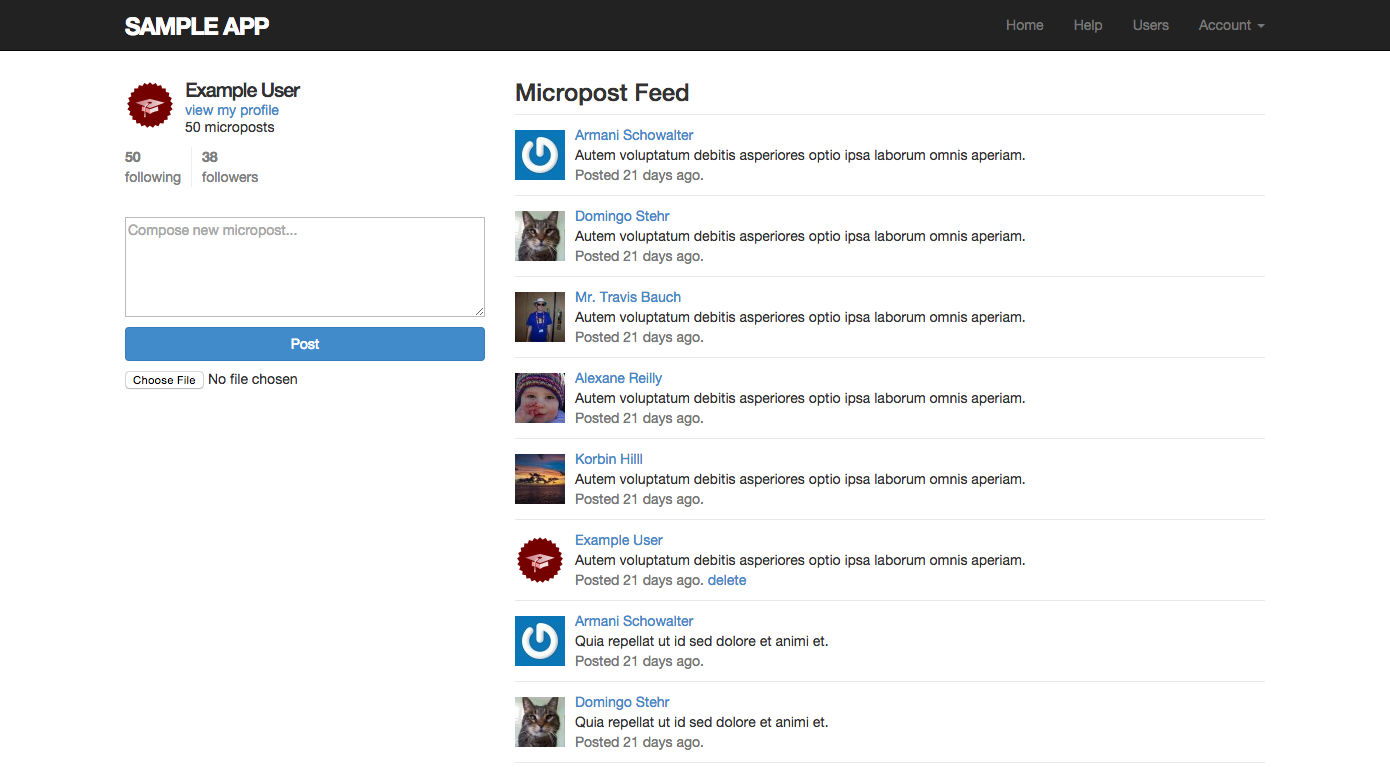
\includegraphics[width=0.8\textwidth]{images/figures/sampleapp.png}
\caption{Aplicación web \kode{sample\_app\_rails\_4}. \label{fig:sampleapp}}
\end{figure}

Tiene una arquitectura de 3 capas: cliente, aplicación y base de datos. Está creada a partir de páginas estáticas con contenido dinámico, tiene un diseño de sitio web, un modelo de datos de usuario y un sistema completo de registro y autenticación, incluida la activación de cuentas y restablecimiento de contraseñas. Además, cuenta con funciones de \textit{microblogging} y redes sociales. 

Así, la aplicación tendrá usuarios que crearán \textit{microposts} dentro de un marco de autenticación e inicio de sesión, donde la interfaz gráfica de la página principal de un usuario concreto se visualizará como muestra la Figura \ref{fig:sampleapp}.

La arquitectura Ruby on Rails de esta aplicación se pueden apreciar en la Figura \ref{fig:architecturesampleapp}.

\begin{figure}[H]
\centering
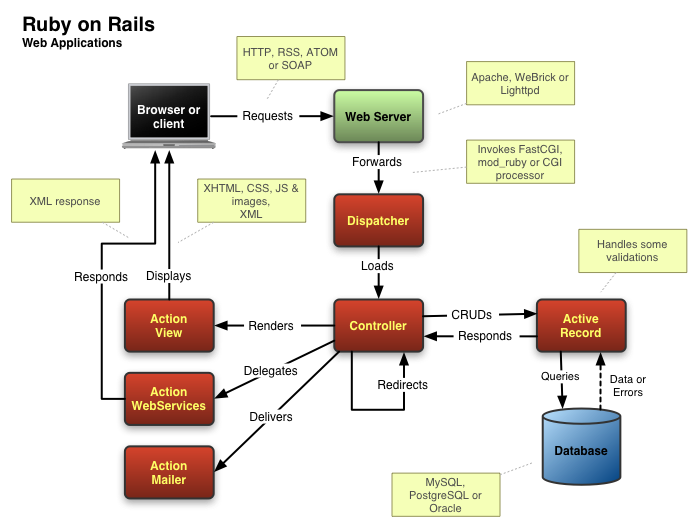
\includegraphics[width=0.7\textwidth]{images/figures/rubyonrails.png}
\caption{Integración entre características y componentes de Ruby on Rails.\footnotemark \label{fig:architecturesampleapp}}
\end{figure}

\footnotetext{Mejia (2011). Ruby on Rails Architectural Design [Figura]. Recuperado de \url{http://adrianmejia.com/blog/2011/08/11/ruby-on-rails-architectural-design}}

Sus características son:
\begin{itemize}
\item Arquitectura Modelo-Vista-Controlador (MVC): Mejora la capacidad de mantenimiento, desacoplamiento y pruebas de la aplicación.
\item Arquitectura \textit{Representational State Transfer} (REST) para servicios web.
\item Soporta las principales bases de datos como MySQL y PostgreSQL.
\item Generadores de \textit{scripts} para automatizar tareas.
\item Uso del formato de serialización de datos \textit{YAML}.
\end{itemize}

Las características se distribuyen en los siguientes componentes de Rails:
\begin{itemize}
\item \textit{Action Mailer}: Proporciona servicios de correo electrónico. 
\item \textit{Action Pack}: Capta las solicitudes de usuario realizadas por el navegador y las asigna a acciones definidas en la capa de controladores.
\subitem-- \textit{Action Controller}: Enruta solicitudes al controlador. 
\subitem-- \textit{Action Dispatcher}: Controla, analiza y procesa el enrutamiento de la solicitud del navegador web.
\subitem-- \textit{Action View}: Realiza la presentación de la página web solicitada.
\item \textit{Active Model}: Define la interfaz entre el \textit{Action Pack} y los módulos \textit{Active Record}.
\item \textit{Active Record}: Proporciona la capacidad de crear relaciones o asociaciones entre modelos y construye la capa Modelo que conecta las tablas de la base de datos con su representación en las clases Ruby.
\item \textit{Active Resource}: Administra la conexión entre servicios web \textit{RESTful} y objetos de negocio.
\item \textit{Active Support}: Colección de clases de utilidad y extensiones de bibliotecas estándar de Ruby útiles para el desarrollo en Ruby on Rails.
\item \textit{Railties}: Código básico de Rails que construye nuevas aplicaciones. 
\end{itemize}	 

Una vez vistas las características y componentes, tanto de una aplicación Ruby on Rails genérica como de la aplicación en actual estudio, se elabora un trabajo adicional a partir de ella, aplicando una serie de cambios y adiciones para la consecución de los objetivos inicialmente propuestos.

\section[Iteración 1: Arquitectura de microservicios]{Iteración 1: Conversión a una arquitectura de microservicios con el uso de Docker}

Como se muestra en la Figura \ref{fig:figure_docker_microservices}, la primera iteración consiste en adecuar la aplicación para que utilice contenedores en su funcionamiento. Esta tarea supone el uso de la tecnología de contenedores Docker para realizar el despliegue, en una máquina física, de la siguiente infraestructura:

\begin{figure}[H]
\image{images/figures/iteration1.png}
\caption{Infraestructura de la aplicación con contenedores Docker.\label{fig:figure_docker_microservices}}
\end{figure}

La aplicación \kode{sample\_app\_rails\_4} está disponible en un repositorio GitHub. Para trabajar con ella se hará una copia del repositorio a través de la opción \textit{fork}. Esto crea una bifurcación que permite la libre experimentación de cambios, sin afectar el proyecto original, utilizando el proyecto de otra persona como punto de partida de una idea propia.

Mediante Docker se obtienen las imágenes pertenecientes a dos servicios. El primero implementa la funcionalidad de la base de datos \kode{PostgreSQL} y el segundo el servidor web y proxy inverso \kode{Nginx}. El proxy inverso es un proxy que aparenta ser un servidor web ante los clientes, pero que en realidad reenvía las solicitudes que recibe a uno o más servidores de origen. Se escoge \kode{Nginx} por ser multiplataforma, ligero, de alto rendimiento y software libre.

La aplicación en su origen utiliza una base de datos \kode{SQLite} que se cambia por \kode{PostgreSQL}, presente en el contenedor \kode{some-postgres}. 

Otro de los cambios a implementar es la sustitución del servidor web \kode{rails s} por \kode{puma}, construido para ofrecer mayor velocidad y paralelismo.

Para poder crear un contenedor que contenga la aplicación web habrá que crear su imagen Docker, que se llamará \kode{sample\_app\_rails\_4\_image}. A efectos de mantenerla remotamente se subirá al repositorio de imágenes Docker Hub con la etiqueta \kode{initial}.

El principal propósito de este despliegue es que pueda realizarse automáticamente tras la ejecución de un \textit{script}. Este fichero comprobará que las variables de entorno que especifican el nombre y la contraseña del usuario de las distintas bases de datos PostgreSQL existentes (test, desarrollo y producción) están correctamente establecidas.

Luego se creará el contenedor \kode{some-postgres} con el servidor \kode{PostgreSQL} y, seguidamente, se creará el contenedor de la aplicación web, llamado \kode{some-app}, a partir de la imagen de ésta, enlazándola con el contenedor \kode{some-postgres}, que será su base de datos.

Con la intención de utilizar como servidor web de la aplicación un contenedor diferente al propio, se crea el contenedor \kode{some-nginx} que proporciona el servidor \kode{Nginx}. Se le indicará que el tráfico del puerto 8080 en el sistema anfitrión se redirija al 80 del contenedor. Así, el sitio web será accesible por la dirección local en el puerto 8080. Además, se enlazará a la aplicación web mediante el contenedor en el que se ejecuta.

También se crea un volumen Docker de datos, llamado \kode{volume-public}, para compartirlo entre la aplicación web, la base de datos y el servidor proxy.

Con todo ello, quedará construir, migrar y poblar la base de datos para, finalmente, ejecutar el servidor \kode{puma} dentro del contenedor \kode{some-app} y comprobar desde el sistema anfitrión que la página principal de la aplicación \kode{sample\_app\_rails\_4} está disponible en el puerto 8080. Esto producirá el resultado de la Figura \ref{fig:resultado1}:

\begin{figure}[H]
\centering
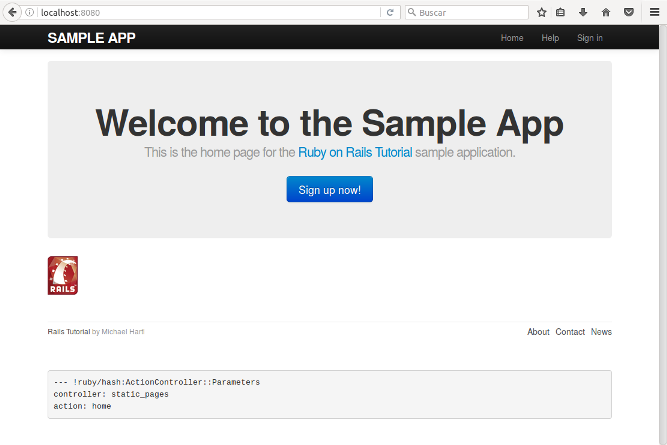
\includegraphics[width=0.7\textwidth]{images/figures/resultado1.png}
\caption{Resultado de la Iteración 1 con el uso de Docker. \label{fig:resultado1}}
\end{figure}

\subsection{Preparación del repositorio local y remoto}

En primer lugar se realiza una copia del repositorio GitHub de la aplicación \kode{sample\_app\_rails\_4}. Para ello se realiza un \textit{fork} seleccionando el botón con el mismo nombre y automáticamente se crea la copia del repositorio en la cuenta personal. Seguidamente se clona esta copia para trabajar localmente:

%= lang:bash
\begin{code}
$ git clone https://github.com/CarolinaSantana/sample_app_rails_4-1.git 
\end{code}

Luego se entra en la carpeta local que lo contiene, seleccionando como \textit{gemset}, conjunto aislado de gemas incorporadas en la aplicación para la versión Ruby en uso, 2.0.0, quedando como \kode{2.0.0@railstutorial\_rails\_4\_0}. Además se deja lista la configuración de base de datos, utilizando la que viene a modo de ejemplo, con la intención de probar que los test que comprueban su funcionalidad pasen positivamente: 

%= lang:bash
\begin{code}
$ cd sample_app_rails_4-1
$ cp config/database.yml.example config/database.yml
$ bundle install --without production
$ bundle exec rake db:migrate
$ bundle exec rake db:test:prepare
$ bundle exec rspec spec/
\end{code}

\subsection{Cambio y configuración de la base de datos} \label{postgrescredentials}

Con la intención de realizar el cambio de la base de datos se elimina del fichero \kode{Gemfile} la gema \kode{sqlite3 1.3.8}, como base de datos en desarrollo, y se cambia por una base de datos PosgreSQL, concretamente la versión \kode{pg 0.15.1}. Para instalar la nueva gema se ejecuta:

%= lang:bash
\begin{code}
$ bundle install --without production
\end{code}

La instalación de \kode{PostgreSQL} requiere credenciales de usuario con contraseña para acceder y se especifica mediante las variables de entorno \kode{\$POSTGRES\_USER} y \kode{\$POSTGRES\_PASSWORD} en el fichero local \kode{\textasciitilde{}/.postgres/credentials}, cuyo contenido es:

\begin{codelisting}
\label{code:credentials}
\codecaption{Fichero \kode{\textasciitilde{}/.postgres/credentials}}
\begin{code}
export POSTGRES_USER=postgres
export POSTGRES_PASSWORD=postgres
\end{code}
\end{codelisting}

Se da permiso de ejecución tanto al fichero como a la carpeta que lo contiene y se exportan las variables de entorno en el directorio de la aplicación:

%= lang:bash
\begin{code}
$ chmod 0700 ~/.postgres
$ chmod 0700 ~/.postgres/credentials
$ . ~/.postgres/credentials
\end{code}

Ahora se cambia el fichero de configuración de la base de datos para que especifique lo siguiente:

\begin{codelisting}
\label{code:database}
\codecaption{Cambios en el fichero \kode{config/database.yml}}
\begin{code}
default: &default
  adapter: postgresql
  encoding: unicode
  pool: 5
  username: <%= ENV['POSTGRES_USER'] %>
  password: <%= ENV['POSTGRES_PASSWORD'] %>
  port: 5432
development:
  <<: *default
  database: sample_app_development  
  host : db
test:
  <<: *default
  database: sample_app_test
  host: db
production:
  <<: *default
  database: sample_app_production
\end{code}
\end{codelisting}

El nombre de usuario y la contraseña de las bases de datos de desarrollo, test y producción se indica con variables de entorno. Además, se especifica que ha de conectarse a \textit{db}, que será el nombre por el que ha de descubrir el contenedor Docker que provisiona el servidor \kode{PostgreSQL}.

Por motivos de seguridad el fichero de configuración de la base de datos no debe subirse al repositorio remoto, por lo que se hace una copia para tener esta configuración de ejemplo:

%= lang:bash
\begin{code}
$ cp config/database.yml config/database.yml.postgres
\end{code}

\subsection{Cambio del alimentador idempotente de base de datos}

Cuando se alimenta la base de datos solo han de crearse datos ella si aún no existen. Para ello se cambia a \textit{seed} idempotente el fichero que viene por defecto, \kode{lib/tasks/sample\_data.rake}, quedando como:

\begin{codelisting}
\label{code:idempotentseed}
\codecaption{Fichero \kode{lib/tasks/sample\_data.rake}}
%= lang:ruby
\begin{code}
namespace :db do
  desc "Fill database with sample data"
  task populate: :environment do
    make_users_microposts_relationships
  end
end
def make_users_microposts_relationships
  User.find_or_create_by(email:"example@railstutorial.org") do |admin|
  	admin.name = "Example User"
	admin.password = "foobar"
        admin.password_confirmation = "foobar"
        admin.admin = true
	99.times do |n|
	    name  = Faker::Name.name
	    email = "example-#{n+1}@railstutorial.org"
	    password  = "password"
	    User.create!(name:     name,
                 email:    email,
                 password: password,
                 password_confirmation: password)
        end
	users = User.all(limit: 6)
  	50.times do
	    content = Faker::Lorem.sentence(5)
	    users.each { |user| user.microposts.create!(content: content) }
	end  
	users = User.all
	user  = users.first
	followed_users = users[2..50]
	followers      = users[3..40]
	followed_users.each { |followed| user.follow!(followed) }
	followers.each      { |follower| follower.follow!(user) }
  end
end
\end{code}
\end{codelisting}

\subsection{Cambio y configuración del servidor web}

Para acceder a la aplicación se escoge cambiar el servidor web \kode{rails s} por \kode{puma}\footnotettt{Servidor Web Puma}{http://puma.io}. Para ello se añade al fichero \kode{Gemfile} la gema \kode{puma} y se instala: 

%= lang:bash
\begin{code}
$ bundle install --without production
\end{code}

\subsection{Configuración para la creación de los contenedores}

En primer lugar se configuran los registros o \textit{logs} que crearán los contenedores añadiendo en el fichero \kode{config/application.rb} lo siguiente:

\begin{codelisting}
\label{code:application.rb}
\codecaption{Fichero \kode{config/application.rb}}
%= lang:ruby
\begin{code}
.
config.logger = Logger.new(STDOUT)
.
\end{code}
\end{codelisting}

Para que la imagen Docker que se construya del repositorio sea más ligera se añade el fichero \kode{.dockerignore}, como copia de \kode{.gitignore}:

\begin{codelisting}
\label{code:.dockerignore}
\codecaption{Fichero \kode{.dockerignore}}
%= lang:ruby
\begin{code}
.
cp .gitignore .dockerignore
.
\end{code}
\end{codelisting}

La creación de los contenedores se lleva a cabo ejecutando el \textit{script} \kode{docker-microservice.sh}.

Primero comprueba que las variables de entorno con el nombre y la contraseña del usuario de la base de datos PostgreSQL están establecidas.

Para crear el contenedor de la aplicación hay que construir su imagen, \kode{sample\_app\_rails\_4\_image}, previamente. El fichero \kode{Dockerfile} especifica cómo crearla, indicando que lo hará a partir de una imagen Ruby y que debe actualizar todos los paquetes e instalar \textit{nodejs}, requerido por la aplicación, y \textit{netcat}, para comprobar que el servicio PostgreSQL está listo, terminando con una limpieza de las capas intermedias. 

La lógica de construcción de la aplicación, basada en su imagen, pasa por la creación de dos contenedores. El primer contenedor, \kode{app-job}, se configurará a partir de un \textit{entrypoint}, llamado \kode{setup.sh}, que va a permitir ejecutar el contenedor como un ejecutable. Este contenedor esperará a que el servicio \textit{PostgreSQL} esté activo en el contenedor \kode{some-postgres} para crear, migrar, alimentar y poblar las bases de datos. Además, la aplicación implementa el modo de autenticación por medio de \textit{tokens}. Cuando el cliente se autentica mediante su usuario y contraseña cada petición HTTP que hace irá acompañada de un \textit{token} en la cabecera, permitiendo que sea identificado. En el actual entorno de desarrollo va a ser utilizado un determinado \textit{token} de prueba. Para ello se realiza la copia del actual \kode{.secret}, localizado en el directorio principal, como \kode{.secret.example}. Luego se incluye como \textit{token} en el fichero. Una vez acaba, el contenedor \kode{app-task} vuelve al estado inactivo. 

\begin{codelisting}
\label{code:dockerfile}
\codecaption{Fichero \kode{setup.sh}}
%= lang:ruby
\begin{code}
#!/bin/sh

cp config/database.yml.postgresql config/database.yml
echo "Waiting PostgreSQL to start on 5432..."
while ! nc -z some-postgres 5432; do
  sleep 0.1
done
echo "PostgreSQL started"
echo "Creating databases..."
rake db:create
cp ./.secret.example ./.secret
echo "Migrating to databases..."
rake db:migrate
echo "Seeding databases..."
rake db:seed
echo "Populating databases..."
rake db:populate
echo "Ready databases"
\end{code}
\end{codelisting}

Así como se tiene el contenedor \textit{job} se necesita un segundo contenedor \textit{task}, llamado \kode{app-task}. Este contenedor se construye tras el anterior.

\begin{codelisting}
\label{code:dockerfile}
\codecaption{Contenido de \kode{Dockerfile}}
%= lang:ruby
\begin{code}
FROM ruby:2.0-onbuild
LABEL sample_app_rails_4_image.version="0.1" 
      sample_app_rails_4_image.release-date="2016-12-10"
MAINTAINER Carolina Santana "c.santanamartel@gmail.com"
RUN apt-get update && apt-get -y install nodejs && \
    apt-get -y install netcat && \
    apt-get autoclean && apt-get clean && \
    rm -rf /var/lib/apt/lists/* && \
    rm -f /tmp/* /var/tmp/*
\end{code}
\end{codelisting}

Con la intención de exportar un volumen compartido entre los contenedores de la aplicación y \kode{some-nginx} para que compartan el directorio \kode{/usr/src/app/public} y el directorio \kode{/var/lib/postgresql} con el contenedor \kode{some-postgres} se crea un volumen Docker llamado \kode{volume-public}.

La siguiente acción es la creación del contenedor \kode{some-postgres} con el servidor \kode{PostgreSQL}, a partir de la imagen \kode{postgres} indicada con \textit{\--d}. Para poder acceder a la base de datos es necesario pasarle las credenciales, con \textit{\--e}. El volumen creado se exporta mediante \textit{\--v}.

Ahora se crea el contenedor \textit{job} de la aplicación web, llamado \kode{app-job}, a partir de la imagen de ésta, \textit{\--d}, indicando como \textit{\---entrypoint} el \textit{script} comentado y enlazando la base de datos de la misma con el contenedor \kode{some-postgres} a través del indicador \textit{\---link}. Además, se le pasan las variables de entorno necesarias para acceder a la base de datos, con \textit{\--e}. Por su parte, el indicador \textit{\--it} ofrece un terminal interactivo dentro del contedor y \textit{\--w} indica que se va a compartir el directorio inicial del proyecto local en el contenedor. El volumen creado se exporta mediante \textit{\--v}.

El siguiente paso crea el contenedor \textit{task} de la aplicación web, llamado \kode{app-task}. Se construye como el anterior sin el \textit{entrypoint}, configurando y preparando las bases de datos, el \textit{token} de prueba y ejecutando el servidor \kode{puma} en el puerto \kode{9292}. Todo ello a través de \textit{/bin/bash \--c}

Para crear el contenedor \kode{some-nginx} que proporciona el servidor Nginx se indica la imagen con \textit{\--d}, que el tráfico del puerto 8080 en el sistema anfitrión se redirija al 80 del contenedor, \textit{\--p}, y se enlaza la aplicación web con el contenedor en el que se ejecuta, a través del indicador \textit{\---link}. Además se monta el volumen \kode{volume-public} con el indicador \textit{\--v}. Por último, se crea localmente el fichero de configuración \kode{/etc/nginx/conf.d/nginx.conf} en el que se especifica que este servidor escuchará en el puerto 80, hará uso del directorio \kode{/usr/src/app/public}, se agregan los campos de redirección y nombre del servidor al encabezado de solicitud, se deshabilita la redirección a otra ruta, se indican los ficheros para el procesamiento de solicitudes, así como que ha de resolver la aplicación en el puerto 9292, usado por \kode{puma}.  

\begin{codelisting}
\label{code:nginxconf}
\codecaption{Fichero \kode{nginx.conf}}
%= lang:java
\begin{code}
server {
  listen 80;
  root /usr/src/app/public;
  location / {
    proxy_set_header X-Forwarded-For $proxy_add_x_forwarded_for;
    proxy_set_header Host $http_host;
    proxy_redirect off;
    try_files $uri /page_cache/$uri /page_cache/$uri.html @app;
  }
  location @app{
    proxy_pass http://app:9292;
    break;
  }
}
\end{code}
\end{codelisting}

El \textit{script} \kode{./docker-microservices.sh}, con permiso \kode{chmod +x} es:

\begin{codelisting}
\label{code:scriptdocker}
\codecaption{Contenido de \kode{docker-microservices.sh}}
%= lang:bash
\begin{code}
#!/bin/bash

if [ "$POSTGRES_USER" = "" ] || [ "$POSTGRES_PASSWORD" = "" ]; then
	echo "Environment variables for POSTGRES not found"
        exit
fi
docker build -t sample_app_rails_4_image .
docker volume create --name volume-public
docker run --name some-postgres -e POSTGRES_USER=$POSTGRES_USER \
  -e POSTGRES_PASSWORD=$POSTGRES_PASSWORD \
  -v volume-public:/var/lib/postgresql -d postgres
docker run -i --name app-job --entrypoint ./setup.sh \
  -e POSTGRES_USER=$POSTGRES_USER -e POSTGRES_PASSWORD=$POSTGRES_PASSWORD \
  -w /usr/src/app -v volume-public:/var/lib/postgresql \
  --link some-postgres:db sample_app_rails_4_image
docker run -d -it --name app-task -e POSTGRES_USER=$POSTGRES_USER \
  -e POSTGRES_PASSWORD=$POSTGRES_PASSWORD -w /usr/src/app \
  -v volume-public:/usr/src/app/public --link some-postgres:db \
  sample_app_rails_4_image \
  /bin/bash -c "cp config/database.yml.postgresql config/database.yml && \
  cp ./.secret.example ./.secret && puma -p 9292"
docker run --name some-nginx \
  -v "${PWD}/nginx.conf":/etc/nginx/conf.d/default.conf \
  -p 8080:80 --link app-task:app -v volume-public:/usr/src/app/public -d nginx
\end{code}
\end{codelisting}

\subsection{Resultado}

El resultado del \textit{script} anterior crea los elementos propuestos en el planteamiento de esta iteración. 

Las imágenes Docker descargadas y creada son:

\begin{figure}[H]
\centering
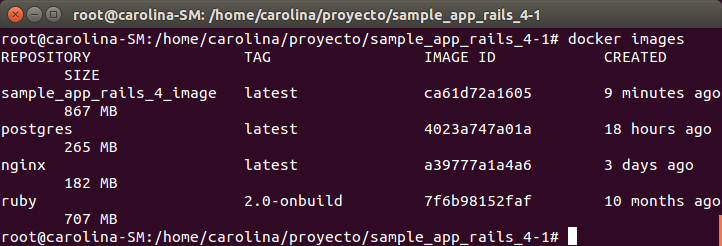
\includegraphics[width=0.7\textwidth]{images/figures/dockerimages.png}
\caption{Imágenes docker mostradas con \kode{docker images}.}
\end{figure}

Los contenedores Docker creados son:

\begin{figure}[H]
\centering
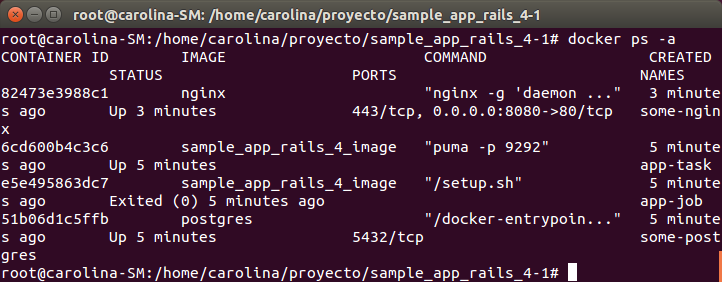
\includegraphics[width=0.7\textwidth]{images/figures/dockerps.png}
\caption{Contenedores docker mostrados con \kode{docker ps -a}.}
\end{figure}

De esta manera, se hace una petición mediante el comando \kode{curl}. El contenedor \kode{some-nginx} la recibirá y redirigirá al contenedor \kode{app-task} donde se encuentra el servidor web de la aplicación:

%= lang:bash
\begin{code}
$ curl http://localhost:8080
\end{code}

\begin{figure}[H]
\centering
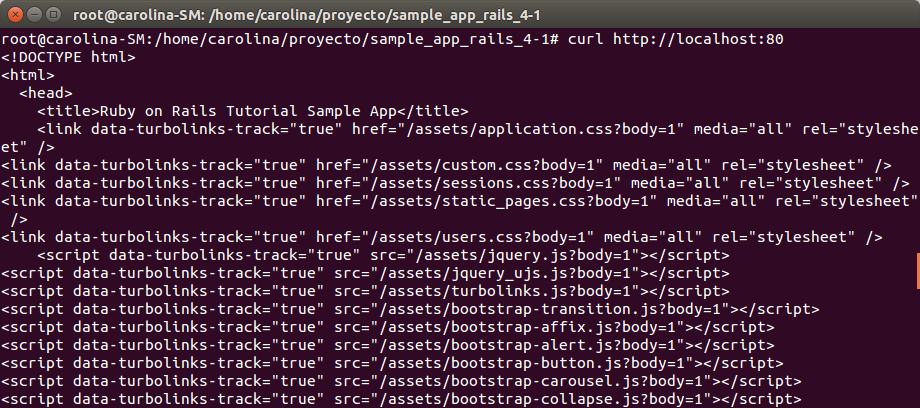
\includegraphics[width=0.8\textwidth]{images/figures/curldocker.png}
\caption{Resultado de la petición \kode{curl http://localhost:8080}.}
\end{figure}

\section[Iteración 2: Subida de la imagen a Docker Hub]{Iteración 2: Subida de la imagen resultante de la aplicación al repositorio de imágenes Docker Hub}

A efectos de mantener la imagen remotamente se sube al repositorio Docker Hub, previa creación de una cuenta en él. Para ello se inicia sesión por consola y se añade una etiqueta a la imagen \kode{sample\_app\_rails\_4\_image}, especificando su identificador y el repositorio escogido dentro de la cuenta:

%= lang:bash
\begin{code}
$ docker login
$ docker tag <image-id> carolina/sample_app_rails_4_image:initial
$ sudo docker push carolina/sample_app_rails_4_image
\end{code}

Puede ser comprobado localmente mediante:

%= lang:bash
\begin{code}
$ docker images carolina/sample_app_rails_4_image:initial
\end{code}

\begin{figure}[H]
\image{images/figures/dockerimages3.png}
\caption{Versión \textit{initial} de la imagen \kode{sample\_a\_rails\_4} en local.}
\end{figure}

La imagen etiquetada como \kode{initial} se aprecia ahora en Docker Hub:

\begin{figure}[H]
\centering
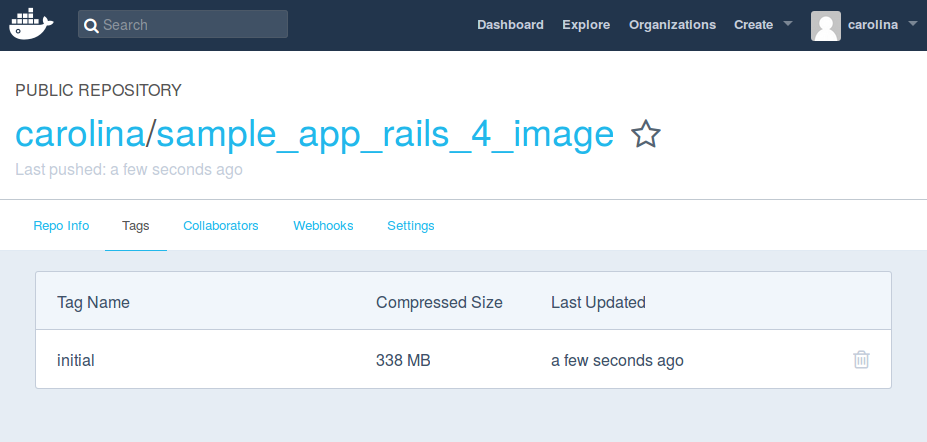
\includegraphics[width=0.8\textwidth]{images/figures/dockerhubinitial.png}
\caption{Versión \textit{initial} de la imagen \kode{sample\_a\_rails\_4} en Docker Hub.}
\end{figure}

\section[Iteración 3: Integración y Despliegue continuos]{Iteración 3: Integración y Despliegue continuos de la aplicación con Travis CI, Docker Hub y GitHub}

En esta iteración se busca adaptar la aplicación Ruby on Rails para que funcione con Travis CI. Esta herramienta se conectará al repositorio de GitHub \kode{sample\_app\_rails\_4-1} con la intención de poder generar una imagen Docker de la aplicación tras cada cambio. Esto permite trabajar en un entorno de desarrollo en el que la integración de los cambios en el proyecto es continua, así como también su despliegue es automatizado.

Para ello se define la estructura presentada en la Figura \ref{fig:iteration2} .
\begin{figure}[H]
\image{images/figures/iteration2.png}
\caption{Integración y Despliegue continuos con Travis CI. \label{fig:iteration2}}
\end{figure}

Las precondiciones, condiciones y postcondiciones necesarias para construir y desplegar la aplicación en uso de manera automática se especifican en el fichero \kode{.travis.yml}. A este fichero se le añadirán, además, las credenciales de la cuenta de Docker Hub y GitHub mediante variables de entorno encriptadas. Las acciones a realizar serán la comprobación de que los tests pasan satisfactoriamente, la construcción de una nueva imagen Docker y su subida al repositorio Docker Hub.

Para llevarlo a cabo es necesario añadir una configuración de base de datos específica. En este caso se llamará \kode{travis\_ci\_test}.

Finalmente, el resultado permitirá que cuando se haga un nuevo cambio o \textit{commit} acompañado de una subida del mismo al repositorio GitHub comenzará, también, la construcción en Travis CI. Tanto en caso de fallo como de éxito se configura el envío de un correo electrónico que lo anuncie. Al repositorio en Docker Hub se subirán 3 copias comprimidas de la imagen. La primera etiquetada con el hash del \textit{commit}, la segunda con el número de construcción en Travis CI y la tercera como la última versión, \textit{latest}:

\begin{figure}[H]
\centering
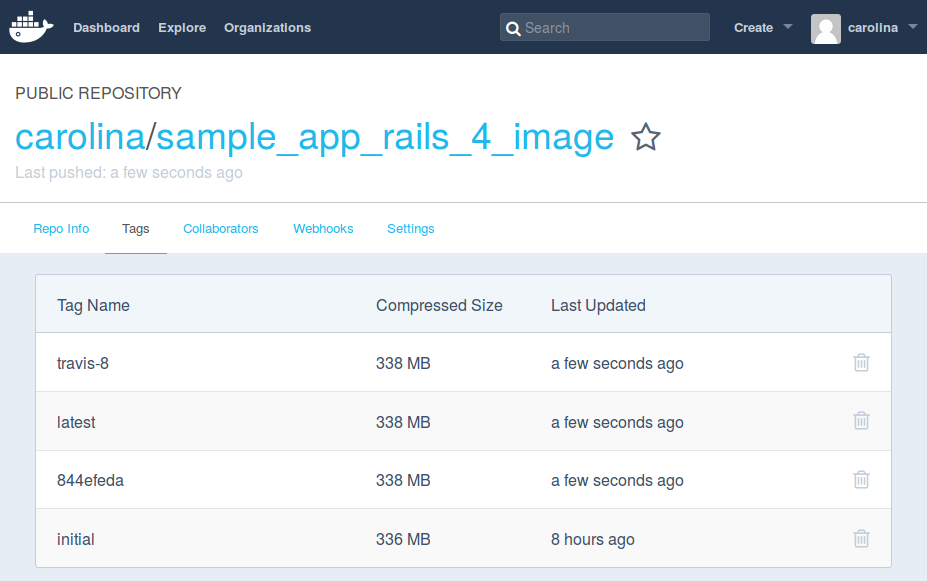
\includegraphics[width=0.7\textwidth]{images/figures/dockerhubimages.png}
\caption{Repositorio de \kode{sample\_app\_rails\_4\_image}.\label{fig:dockerhub_images}}
\end{figure}

\subsection{Vinculación con el repositorio remoto}

En primer lugar hay que ingresar en el sitio Travis CI con la cuenta de GitHub y añadir el repositorio con el que se trabaja actualmente:

\begin{figure}[H]
\centering
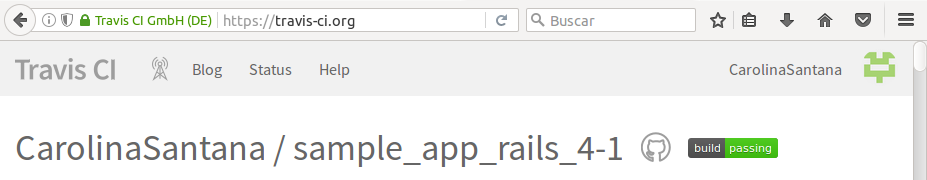
\includegraphics[width=0.7\textwidth]{images/figures/travis_github.png}
\caption{Vinculación de GitHub con Travis CI.\label{fig:travis_github}}
\end{figure}

\subsection{Configuración de condiciones}

En segundo lugar se procede a instalar la gema \kode{travis}. Para ello se edita el fichero \kode{Gemfile}, incluyéndola en el grupo de desarrollo y test.

Luego se instala mediante:

%= lang:bash
\begin{code}
$ bundle install --without production
\end{code}

Para probar el correcto funcionamiento es necesario crear un nuevo fichero de configuración para la base de datos en Travis CI:

\begin{codelisting}
\label{code:travisdatabase}
\codecaption{Fichero \kode{config/database.yml.travis} }
%= lang:ruby
\begin{code}
test:
  adapter: postgresql
  database: travis_ci_test
  username: postgres
\end{code}
\end{codelisting}

Para configurar Travis CI se crea el fichero \kode{.travis.yml}. 

%= lang:bash
\begin{code}
$ touch .travis.yml
\end{code}

Tras ello, se establecen las variables de entorno de las credenciales de Docker Hub. Esto se especifica localmente mediante los comandos:

%= lang:bash
\begin{code}
$ travis env set DOCKER_USERNAME carolina
$ travis env set DOCKER_PASSWORD **************
\end{code}

También se agrega una variable de entorno que contenga los 8 primeros caracteres del \textit{hash} del \textit{git commit}, justo debajo de las anteriores.

En la sección \kode{after\_success} del fichero se inicia sesión en Docker Hub y luego se construye la imagen. Al repositorio en Docker Hub se subirán 3 copias comprimidas de la imagen. La primera etiquetada con el hash del \textit{commit} correspondiente, la segunda con el número de construcción en Travis CI y la tercera como la última versión, \textit{latest}. Además se le indica la base de datos de prueba para la ejecución de los tests y la versión de Ruby en uso.

\begin{codelisting}
\label{code:travis}
\codecaption{Fichero \kode{.travis.yml} }
%= lang:ruby
\begin{code}
env:
  global:
  - COMMIT=${TRAVIS_COMMIT::8}
language: ruby
rvm:
- 2.0.0-p648
bundler_args: --without production
addons:
  postgresql: '9.3'
services:
- docker
before_script:
- cp config/database.yml.travis config/database.yml
- psql -c 'create database travis_ci_test;' -U postgres
- RAILS_ENV=test bundle exec rake db:migrate --trace
script:
- bundle exec rspec
notifications:
  email:
    recipients:
    - c.santanamartel@gmail.com
    on_success: always
    on_failure: always
sudo: required
after_success:
- docker login -u $DOCKER_USERNAME -p $DOCKER_PASSWORD
- export REPO=$DOCKER_USERNAME/sample_app_rails_4_image
- docker build -f Dockerfile -t $REPO:$COMMIT .
- docker tag $REPO:$COMMIT $REPO:latest
- docker tag $REPO:$COMMIT $REPO:travis-$TRAVIS_BUILD_NUMBER
- docker push $REPO  
\end{code}
\end{codelisting}

\subsection{Resultado}

Finalmente, cuando se haga un nuevo \textit{commit} y subida al repositorio GitHub comenzará también la construcción en Travis CI. Tanto si se produce un fallo como si termina con éxito se ha configurado el envío de un correo electrónico para informarlo. 

A continuación, se prueba el caso de fallo comentando la línea que crea la base de datos de prueba \kode{travis\_ci\_test} y el de éxito con ella. Los correos electrónicos recibidos son:

\begin{figure}[H]
\centering
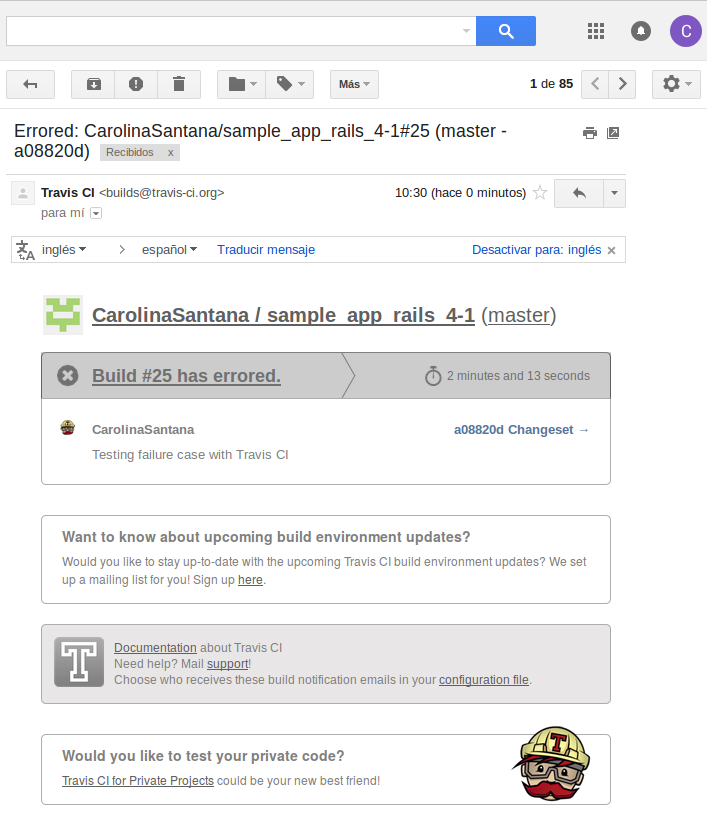
\includegraphics[width=0.6\textwidth]{images/figures/travisfailure.png}
\caption{Correo electrónico de Travis CI en caso de fallo.}
\end{figure}

\begin{figure}[H]
\centering
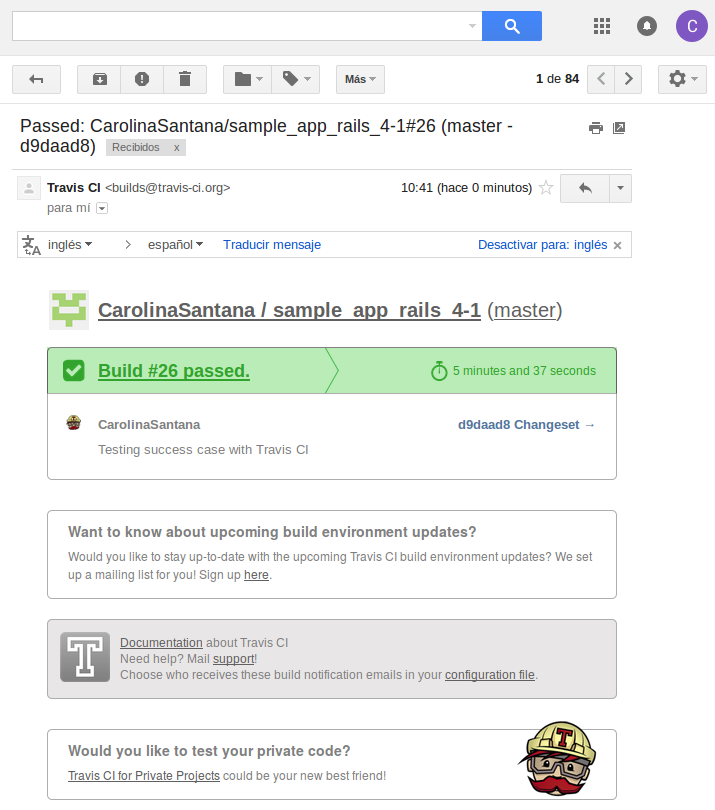
\includegraphics[width=0.6\textwidth]{images/figures/travissuccess.png}
\caption{Correo electrónico de Travis CI en caso de éxito.}
\end{figure}

Dirigiendo a Travis CI donde se comenta el fallo o el éxito:

\begin{figure}[H]
\centering
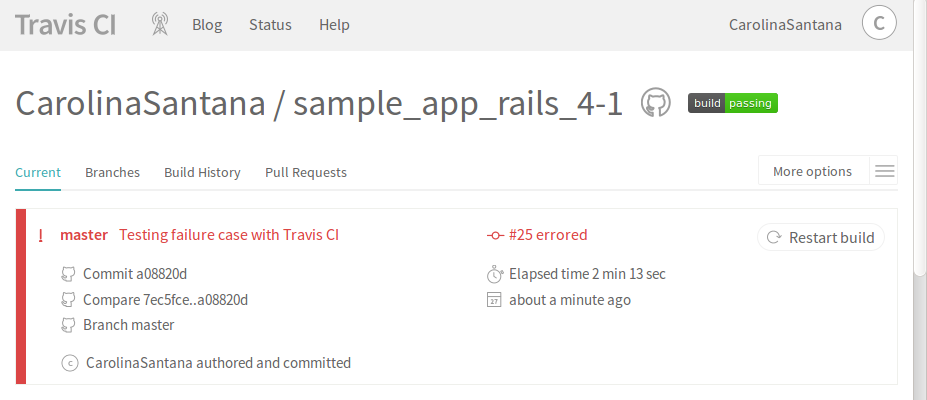
\includegraphics[width=0.7\textwidth]{images/figures/travisfailure2.png}
\caption{Caso de fallo en Travis CI.}
\end{figure}

\begin{figure}[H]
\centering
\image{images/figures/travisfailure3.png}
\caption{Motivo de fallo en Travis CI.}
\end{figure}

\begin{figure}[H]
\centering
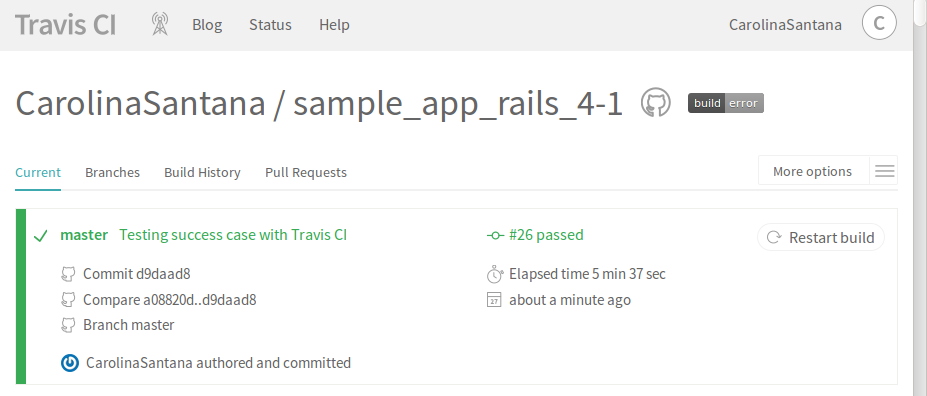
\includegraphics[width=0.7\textwidth]{images/figures/travissuccess2.png}
\caption{Caso de éxito en Travis CI.}
\end{figure}

Esta construcción terminará con la creación y subida de las tres imágenes, comentadas en el planteamiento de esta iteración, en el repositorio de Docker Hub.

\section[Iteración 4: Despliegue en VirtualBox]{Iteración 4: Despliegue monomáquina con unidades de servicio usando Vagrant, VirtualBox y CoreOS}

En esta nueva iteración se aplica el uso del sistema operativo orientado a contenedores CoreOS. De esta manera se crearán unidades de servicio \kode{systemd} que permitirán la correcta aplicación y funcionamiento de los contenedores Docker en los que se divide la aplicación. La infraestructura del nuevo planteamiento es la siguiente:

\begin{figure}[H] 
\centering
\image{images/figures/coreosdiagram.png}
\caption{Infraestructura de la aplicación con unidades de servicio CoreOS.\label{fig:coreosdiagram}}
\end{figure}

En local existen dos herramientas de línea de comandos llamadas \kode{fleectl} y \kode{etcdctl} utilizadas internamente para comunicarse con los elementos del sistema CoreOS \kode{fleetd} y \kode{etcd}. Fleet se encarga de dotar a la máquina CoreOS con los servicios que se desean implementar. Etcd2 permite almacenar los datos de las máquinas CoreOS.

Para llevar a cabo esta iteración se utiliza el repositorio GitHub \kode{coreos/coreos-vagrant} que proporciona una plantilla \kode{Vagrantfile} para configurar el entorno de una máquina virtual CoreOS, usando el hipervisor software VirtualBox.

En este procedimiento se utilizan tres archivos relevantes que se describirán a lo largo del proceso. De esta forma se utilizará la misma configuración para el fichero \kode{config.rb}, se creará un nuevo \kode{cloud-config} que será llamado \kode{user-data.sampleapp.vbox} y se modificará el fichero \kode{Vagranfile}.

\subsection{Preparación del repositorio local y remoto}

En primer lugar se realiza un \textit{fork} del repositorio \kode{coreos/coreos-vagrant} seleccionando el botón con el mismo nombre. Automáticamente se crea la copia en la cuenta personal y se clona para trabajar localmente:

%= lang:bash
\begin{code}
$ git clone https://github.com/CarolinaSantana/coreos-vagrant.git 
\end{code}

Luego, se accede a la carpeta local que lo contiene y se prepara para comprobar su funcionamiento con los datos de usuario y la configuración de ejemplo. Esto se prueba ejecutando el \kode{Vagrantfile} y conectándose a la máquina virtual creada. En este caso se utiliza VirtualBox, lo que se conseguiría con \kode{vagrant up ---provider=virtualbox} o \kode{vagrant up}, puesto que es el proveedor por defecto. 

%= lang:bash
\begin{code}
$ cd coreos-vagrant
$ cp user-data.sample user-data
$ cp config.rb.sample config.rb
$ vagrant up
$ vagrant ssh core-01
\end{code}

Comprobando que funciona correctamente:

\begin{figure}[H]
\centering
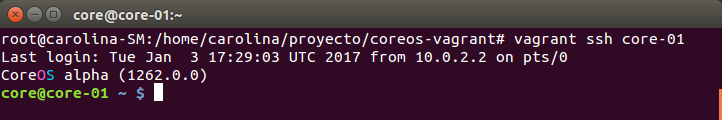
\includegraphics[width=0.7\textwidth]{images/figures/vagrantssh.png}
\caption{Conexión ssh a la máquina virtual \kode{core-01}.}
\end{figure}

Además puede visualizarse la máquina mediante VirtualBox:

\begin{figure}[H]
\centering
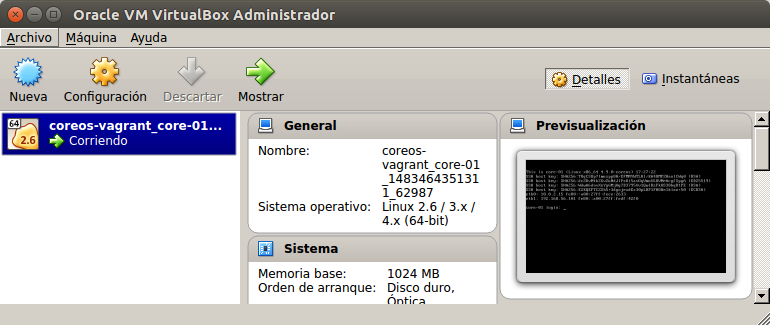
\includegraphics[width=0.6\textwidth]{images/figures/vboxcore01.png}
\caption{Máquina virtual \kode{core-01} desde VirtualBox.}
\end{figure}

\subsection{Preparación de la cabecera del fichero user-data}

El fichero \kode{user-data} es el archivo de configuración \kode{cloud-config}. Especifica el \textit{discovery token} que forma parte de la \textit{URL} de descubrimiento que conecta las instancias. También indica las variables de entorno y la lista de unidades de servicio que se deben iniciar de forma predeterminada. Los parámetros \kode{coreos.etcd}, \kode{coreos.fleet} y \kode{coreos.flannel} son traducidos a una unidad \kode{systemd} parcial actuando como un archivo de configuración \kode{etcd2}, \kode{fleet} y \kode{flannel}, respectivamente. 

Como el entorno de plataforma admite la función de plantilla de \kode{coreos-cloudinit}, es posible automatizar la configuración de \kode{etcd2} con los campos \kode{\$private\_ipv4} y \kode{\$public\_ipv4}. Al generar un \textit{discovery token} se establece el tamaño del clúster, ya que \kode{etcd2} lo utiliza para determinar si todos los miembros se han unido a él. Después de inicializarse, el clúster puede crecer o reducirse. Por su parte \kode{fleet} y \kode{flannel} usan variables de entorno en su configuración.

La siguiente sección de este fichero pertenece a las unidades de servicio, de las que ya se encuentran definidas \kode{etcd2.service}, \kode{fleet.service}, \kode{flanneld.service}, donde esta última especifica la red en CoreOS, siendo utilizada la 10.1.0.0/16 como pública para los contenedores, y \kode{docker-tcp.socket}, el cual permite que se pueda usar el servicio \kode{docker-service} dentro de cada máquina.

CoreOS posee la opción de actualizar automáticamente el sistema operativo cuando una actualización es detectada o la opción de que no sean reiniciadas con la intención de que lo haga el usuario. Como se está en un entorno de desarrollo se escoge la segunda opción.

\begin{codelisting}
\label{code:cloud-config1}
\codecaption{Fichero \kode{user-data}}
%= lang:yaml
\begin{code}
#cloud-config
---
coreos:
  update:
    reboot-strategy: "off"
  etcd2:
    advertise-client-urls: http://$public_ipv4:2379
    initial-advertise-peer-urls: http://$private_ipv4:2380
    listen-client-urls: http://0.0.0.0:2379,http://0.0.0.0:4001
    listen-peer-urls: http://$private_ipv4:2380,http://$private_ipv4:7001
    discovery: https://discovery.etcd.io/acd611cb07df434a400bbd7e36d793a0
  fleet:
    public-ip: "$public_ipv4"
  flannel:
    interface: "$public_ipv4"
  units:
  - name: etcd2.service
    command: start
  - name: fleet.service
    command: start
  - name: flanneld.service
    drop-ins:
    - name: 50-network-config.conf
      content: |
        [Service]
        ExecStartPre=/usr/bin/etcdctl set /coreos.com/network/config \
        '{ "Network": "10.1.0.0/16" }'
    command: start
  - name: docker-tcp.socket
    command: start
    enable: true
    content: |
      [Unit]
      Description=Docker Socket for the API
      [Socket]
      ListenStream=2375
      Service=docker.service
      BindIPv6Only=both
      [Install]
      WantedBy=sockets.target
\end{code}
\end{codelisting}

\subsection{Interpretación del fichero config.rb}

El segundo fichero importante para este despliegue es \kode{config.rb}. Especifica el número de nodos CoreOS y proporciona una opción para generar automáticamente el \textit{discovery token}, valor que se reemplaza automáticamente cuando se inicia el despliegue o levantamiento de una máquina. Además permite la necesaria corrección del valor del parámetro perteneciente a la estrategia de reinicio de CoreOS, al tener que ser la entrada en el fichero \kode{user-data} de una manera distinta a como es traducido por YAML.

\begin{codelisting}
\label{code:cloud-config1}
\codecaption{Fichero \kode{config.rb}}
%= lang:ruby
\begin{code}
$num_instances=1
$new_discovery_url="https://discovery.etcd.io/new?size=#{$num_instances}"
if File.exists?('user-data') && ARGV[0].eql?('up')
  require 'open-uri'
  require 'yaml'
  token = open($new_discovery_url).read
  data = YAML.load(IO.readlines('user-data')[1..-1].join)
  if data.key? 'coreos' and data['coreos'].key? 'etcd'
    data['coreos']['etcd']['discovery'] = token
  end
  if data.key? 'coreos' and data['coreos'].key? 'etcd2'
    data['coreos']['etcd2']['discovery'] = token
  end
  # Fix for YAML.load() converting reboot-strategy from 'off' to `false`
  if data.key? 'coreos' and data['coreos'].key? 'update' 
    and data['coreos']['update'].key? 'reboot-strategy'
    if data['coreos']['update']['reboot-strategy'] == false
      data['coreos']['update']['reboot-strategy'] = 'off'
    end
  end
  yaml = YAML.dump(data)
  File.open('user-data', 'w') { |file| file.write("#cloud-config\n\n#{yaml}") }
end
\end{code}
\end{codelisting}

\subsection{Preparación del fichero Vagrantfile}

El fichero viene preparado para el uso de los proveedores VirtualBox y VMware. Al no utilizar el segundo se prescinde de sus configuraciones y se reagrupan las instrucciones pertinentes a VirtualBox.

El fichero \kode{Vagrantfile} establece el número de máquinas CoreOS que ha de ser creado por Vagrant. En este caso una sola instancia. Otras especificaciones son las opciones de configuración por defecto a utilizar para crear las máquinas y la imagen a partir de la que hacerlo. El fichero viene preparado para aplicar la redirección de puertos de la máquina virtual al sistema anfitrión. Las direcciónes IP que tomarán las máquinas en la red privada empezarán en 172.17.8.10X. Además, se facilita la opción para habilitar el almacenamiento compartido entre anfitrión y máquina. En último lugar se realiza la copia de la configuración del \kode{user-data} en \kode{/var/lib/coreos-vagrant/vagrantfile-user-data}, dentro de la máquina virtual. Así, \kode{coreos-cloudinit} lee \kode{vagrantfile-user-data} en cada incio y lo utiliza para crear y reproducir lo que indica.

\begin{codelisting}
\label{code:cloud-config1}
\codecaption{Fichero \kode{Vagrantfile}}
%= lang:ruby
\begin{code}
# -*- mode: ruby -*-
# # vi: set ft=ruby :
require 'fileutils'
Vagrant.require_version ">= 1.6.0"
if (!ARGV.nil? && ARGV.join('').include?('provider=virtualbox')) || 
   (!ARGV.nil? && !ARGV.join('').include?('provider'))
  FileUtils.cp_r(File.join(File.dirname(__FILE__), "user-data.sampleapp.vbox"),
  File.join(File.dirname(__FILE__), "user-data"), :remove_destination => true)
end
CLOUD_CONFIG_PATH = File.join(File.dirname(__FILE__), "user-data")
CONFIG = File.join(File.dirname(__FILE__), "config.rb")
$num_instances = 1
$instance_name_prefix = "core"
$update_channel = "alpha"
$image_version = "current"
$vm_gui = false
$vm_memory = 1024
$vm_cpus = 1
$vb_cpuexecutioncap = 100
$shared_folders = {}
$forwarded_ports = {}
if ENV["NUM_INSTANCES"].to_i > 0 && ENV["NUM_INSTANCES"]
  $num_instances = ENV["NUM_INSTANCES"].to_i
end
if File.exist?(CONFIG)
  require CONFIG
end
def vm_gui
  $vb_gui.nil? ? $vm_gui : $vb_gui
end
def vm_memory
  $vb_memory.nil? ? $vm_memory : $vb_memory
end
def vm_cpus
  $vb_cpus.nil? ? $vm_cpus : $vb_cpus
end
Vagrant.configure("2") do |config|
  config.ssh.insert_key = false
  config.ssh.forward_agent = true
  config.vm.box = "coreos-%s" % $update_channel
  if $image_version != "current"
      config.vm.box_version = $image_version
  end
  config.vm.provider :virtualbox do |vb, override|
    override.vm.box_url = "https://storage.googleapis.com/%s.release.core-os.net/
    amd64-usr/%s/coreos_production_vagrant.json" %
    [$update_channel,$image_version]
    vb.check_guest_additions = false
    vb.functional_vboxsf     = false
  end
  if Vagrant.has_plugin?("vagrant-vbguest") then
    config.vbguest.auto_update = false
  end
  (1..$num_instances).each do |i|
    config.vm.define vm_name = "%s-%02d" % [$instance_name_prefix, i] do |config|
      config.vm.hostname = vm_name
      config.vm.provider :virtualbox do |vb, override|
        $forwarded_ports.each do |guest, host|
          override.vm.network "forwarded_port", guest: guest, host: host, 
          auto_correct: true
        end
        vb.gui = vm_gui
        vb.memory = vm_memory
        vb.cpus = vm_cpus
        vb.customize ["modifyvm", :id, "--cpuexecutioncap", 
                      "#{$vb_cpuexecutioncap}"]
        ip = "172.17.8.#{i+100}"
        override.vm.network :private_network, ip: ip
      end
      config.vm.provider :virtualbox do |vb, override|
        # Uncomment below to enable NFS for sharing the host machine into the VM.
        #override.vm.synced_folder ".", "/home/core/share", id: "core", 
        #:nfs => true, :mount_options => ['nolock,vers=3,udp']
        $shared_folders.each_with_index do |(host_folder, guest_folder), index|
          override.vm.synced_folder host_folder.to_s, guest_folder.to_s, 
          id: "core-share%02d" % index, nfs: true, 
          mount_options: ['nolock,vers=3,udp']
        end
      end
      if File.exist?(CLOUD_CONFIG_PATH) && ARGV[0].eql?('up')
        config.vm.provider :virtualbox do |vb, override|
          override.vm.provision :file, :source => "#{CLOUD_CONFIG_PATH}", 
          :destination => "/tmp/vagrantfile-user-data"
          override.vm.provision :shell, :inline => "mv /tmp/vagrantfile-user-data 
          /var/lib/coreos-vagrant/", :privileged => true
        end
      end
    end
  end
end
\end{code}
\end{codelisting}

\subsection{Despliegue manual de las unidades systemd}

El primer paso consiste en permitir que exista almacenamiento NFS compartido entre la máquina local y la máquina virtual CoreOS, para pasar a esta última las unidades de servicio a implementar. Para ello es necesario descomentar la siguiente línea, dentro del fichero \kode{Vagrantfile}:

\begin{codelisting}
\label{code:vagrantfile2}
\codecaption{Fichero \kode{Vagrantfile}}
%= lang:ruby
\begin{code}
.
override.vm.synced_folder ".", "/home/core/share", id: "core", :nfs => true, \
:mount_options => ['nolock,vers=3,udp']
.
\end{code}
\end{codelisting}

También será necesario instalar el adaptador NFS en el sistema anfitrión y cargar los cambios. Esto creará, dentro de la máquina virtual, el directorio \kode{share}, compartido con el sistema anfitrión:

%= lang:bash
\begin{code}
$ sudo apt-get install nfs-kernel-server -y
$ vagrant reload --provision
\end{code}

\subsubsection{Unidad volume-public.service}

La primera unidad de servicio será el volumen Docker compartido entre los contenedores. Se crea la ruta \kode{etc/sysctl/volume-public.service}. En este fichero se configura el servicio \kode{volume-public.service}. Su contenido especifica que comenzará después de que lo haga el servicio Docker, requerido para su funcionamiento. El servicio empezará directamente creando el volumen, añadiendo un enlace simbólico al mismo para todos los usuarios de la máquina. 

\begin{codelisting}
\label{code:volume-public.service}
\codecaption{Fichero \kode{etc/sysctl/volume-public.service}.}
%= lang:ruby
\begin{code}
[Unit] 
  Description= volume-public share between some-postgres, app-job, app-task and 
               some-nginx 
  After=docker.service
  Requires=docker.service
[Service] 
  TimeoutStartSec=0 
  ExecStart=/usr/bin/docker volume create --name volume-public
[Install] 
  WantedBy=multi-user.target
\end{code}
\end{codelisting}

\subsubsection{Unidad postgresql.service}

La siguiente es la unidad de servicio correspondiente a la base de datos de la aplicación. Para ello se crea la ruta \kode{etc/sysctl/postgresql.service}. En este fichero se configura el servicio \kode{postgresql.service}. Se especifica que comenzará después del servicio Docker y \kode{volume-public.service}, requeridos para el correcto funcionamiento. Empezará directamente sin tiempo de espera, se reiniciará siempre si ocurre algún problema y se le indica el fichero del que leer las variables de entorno. Si este servicio ya se ha ejecutado con anterioridad se procederá terminándolo y eliminando el contenedor. Seguidamente, se comprobará, si ya existe la imagen del contenedor en la máquina, que sea la última versión disponible, de no ser así se obtendrá de nuevo. Llegado este punto la unidad de servicio comenzará creando el contenedor, especificando la opción a realizar si quiere pararse. Además se añade un enlace simbólico al mismo para todos los usuarios de la máquina. 

\begin{codelisting}
\label{code:postgresql.service}
\codecaption{Fichero \kode{etc/sysctl/postgresql.service}.}
%= lang:ruby
\begin{code}
[Unit] 
  Description=PostgreSQL database 
  After=docker.service volume-public.service
  Requires=docker.service volume-public.service
[Service] 
  TimeoutStartSec=0
  Restart=always
  EnvironmentFile=/home/core/share/etc/sysctl/postgres-credentials.env
  ExecStartPre=-/usr/bin/docker kill some-postgres 
  ExecStartPre=-/usr/bin/docker rm some-postgres 
  ExecStartPre=/usr/bin/docker pull postgres 
  ExecStart=/usr/bin/docker run --rm --name some-postgres \
  -e "POSTGRES_USER=${POSTGRES_USER}" \
  -e "POSTGRES_PASSWORD=${POSTGRES_PASSWORD}" \
  -v "volume-public:/var/lib/postgresql" -p "5432:5432" postgres 
  ExecStop=/usr/bin/docker stop some-postgres 
[Install] 
  WantedBy=multi-user.target
\end{code}
\end{codelisting}

El contenido del fichero que especifica las variables de entorno hace referencia a las credenciales de la base de datos.

\begin{codelisting}
\label{code:credentials}
\codecaption{Contenido del fichero \kode{/etc/postgres-credentials.env}}
\begin{code}
POSTGRES_USER=postgres
POSTGRES_PASSWORD=postgres
\end{code}
\end{codelisting}

\subsubsection{Unidad app-job.service}

La siguiente unidad de servicio será el contenedor ejecutable de la aplicación que crea, migra y alimenta la base de datos. Para ello se crea la ruta \kode{etc/sysctl/app-job.service}. En este fichero se configura el servicio \kode{app-job.service}. Se especifica que comenzará después de que lo haga el servicio Docker, \kode{volume-public.service} y \kode{postgresql.service}, requeridos para el correcto funcionamiento. Empezará directamente sin tiempo de espera, indicándole el fichero del que leer las variables de entorno necesarias. Si este servicio ya se ha ejecutado con anterioridad se procederá terminándolo y eliminando el contenedor. Seguidamente, se comprobará, si ya existe la imagen del contenedor en la máquina, que sea la última versión disponible, de no ser así se obtendrá de nuevo. La unidad de servicio comenzará creando el contenedor, especificando la opción a realizar si quiere pararse. Además se añade un enlace simbólico al mismo para todos los usuarios de la máquina. 

\begin{codelisting}
\label{code:app-job.service}
\codecaption{Fichero \kode{etc/sysctl/app-job.service}.}
%= lang:ruby
\begin{code}
[Unit] 
  Description=executable app-job container that creates, migrates, seeds and 
              populates the database
  After=docker.service volume-public.service postgresql.service
  Requires=docker.service volume-public.service postgresql.service
[Service] 
  TimeoutStartSec=0 
  EnvironmentFile=/home/core/share/etc/sysctl/postgres-credentials.env
  ExecStartPre=-/usr/bin/docker kill app-job 
  ExecStartPre=-/usr/bin/docker rm app-job 
  ExecStartPre=/usr/bin/docker pull carolina/sample_app_rails_4_image:latest 
  ExecStart=/usr/bin/docker run --rm --name app-job \
  -v "volume-public:/usr/src/app/public" --entrypoint "./setup.sh" \
  -e "POSTGRES_USER=${POSTGRES_USER}" \
  -e "POSTGRES_PASSWORD=${POSTGRES_PASSWORD}" \
  -w "/usr/src/app" --link "some-postgres:db" \
  carolina/sample_app_rails_4_image:latest
[Install] 
  WantedBy=multi-user.target
\end{code}
\end{codelisting}

\subsubsection{Unidad app-task.service}

La siguiente unidad de servicio será el contenedor de la aplicación que ejecuta el servidor puma. Se crea la ruta \kode{etc/sysctl/app-task.service}. En este fichero se configura el servicio \kode{app-task.service}. El contenido del mismo especifica que comenzará después de que lo haga el servicio Docker, \kode{volume-public.service}, \kode{postgresql.service} y \kode{app-job.service}, requeridos para el correcto funcionamiento. El servicio empezará  sin tiempo de espera, se reiniciará si falla y se le indica el fichero del que leer las variables de entorno necesarias. Si este servicio ya se ha ejecutado con anterioridad se procederá terminándolo y eliminando el contenedor. Seguidamente, se comprobará, si ya existe la imagen del contenedor en la máquina, que sea la última versión disponible, de no ser así se obtendrá de nuevo. Llegado este punto la unidad de servicio comenzará creando el contenedor, especificando la opción a realizar si quiere pararse. Además se añade un enlace simbólico al mismo para todos los usuarios de la máquina. 

\begin{codelisting}
\label{code:app-task.service}
\codecaption{Fichero \kode{etc/sysctl/app-task.service}.}
%= lang:ruby
\begin{code}
[Unit] 
  Description=app-task container that runs the server puma
  After=docker.service volume-public.service postgresql.service app-job.service
  Requires=docker.service volume-public.service postgresql.service app-job.service
[Service] 
  TimeoutStartSec=0
  Restart=always 
  EnvironmentFile=/home/core/share/etc/sysctl/postgres-credentials.env
  ExecStartPre=-/usr/bin/docker kill app-task 
  ExecStartPre=-/usr/bin/docker rm app-task
  ExecStartPre=/usr/bin/docker pull carolina/sample_app_rails_4_image:latest 
  ExecStart=/usr/bin/docker run --rm --name app-task \
  -e "POSTGRES_USER=${POSTGRES_USER}" \
  -e "POSTGRES_PASSWORD=${POSTGRES_PASSWORD}" \
  -w "/usr/src/app" -v "volume-public:/usr/src/app/public" \
  --link "some-postgres:db" carolina/sample_app_rails_4_image:latest \
  /bin/bash -c "cp config/database.yml.postgresql config/database.yml && \
  cp ./.secret.example ./.secret && puma -p 9292"
  ExecStop=/usr/bin/docker stop app-task
[Install] 
  WantedBy=multi-user.target
\end{code}
\end{codelisting}

\subsubsection{Unidad nginx.service}

La siguiente unidad del servicio será el contenedor que ejecuta el servidor Nginx. Para ello se crea la ruta \kode{etc/sysctl/nginx.service}. En este fichero se configura el servicio \kode{nginx.service}. El contenido del mismo especifica que comenzará después de que lo haga el servicio Docker, \kode{volume-public.service}, \kode{postgresql.service}, \kode{app-job.service} y \kode{app-task.service}, requeridos para el correcto funcionamiento. El servicio empezará directamente sin tiempo de espera y se reiniciará si falla. Si ya se ha ejecutado con anterioridad se procederá terminándolo y eliminando el contenedor. Seguidamente, se comprobará, si ya existe la imagen del contenedor en la máquina, que sea la última versión disponible, de no ser así se obtendrá de nuevo. La unidad de servicio comenzará creando el contenedor, teniendo en cuenta que ahora la redirección de puertos se ha establecido para trabajar el puerto 80 de la máquina CoreOS con el puerto 80 de la aplicación, especificando la opción a realizar si dicho contenedor quiere pararse. Además se añade un enlace simbólico al mismo para todos los usuarios de la máquina. 

\begin{codelisting}
\label{code:nginx.service}
\codecaption{Fichero \kode{etc/sysctl/nginx.service}.}
%= lang:ruby
\begin{code}
[Unit] 
  Description=some-nginx container that runs a reverse proxy server and a 
              web server
  After=docker.service volume-public.service postgresql.service app-job.service 
        app-task.service
  Requires=docker.service volume-public.service postgresql.service 
           app-job.service app-task.service
[Service] 
  TimeoutStartSec=0
  Restart=always 
  ExecStartPre=-/usr/bin/docker kill some-nginx 
  ExecStartPre=-/usr/bin/docker rm some-nginx
  ExecStartPre=/usr/bin/docker pull nginx 
  ExecStart=/usr/bin/docker run --rm --name some-nginx \
  -v "/home/core/share/etc/sysctl/nginx.conf:/etc/nginx/conf.d/default.conf" \
  -p "80:80" --link "app-task:app" -v "volume-public:/usr/src/app/public" nginx 
  ExecStop=/usr/bin/docker stop some-nginx
[Install] 
  WantedBy=multi-user.target
\end{code}
\end{codelisting}

\subsubsection{Despliegue manual}

Una vez que ya se han configurado y escrito las 5 unidades de servicio necesarias el siguiente paso es preparar su despliegue. Para el reconocimiento de las unidades éstas tienen que ubicarse bajo \kode{systemd}, por lo que se copian al directorio \kode{/etc/systemd/system/}. El funcionamiento de las unidades pasa por dos estados. El primero es la habilitación del servicio, creando el enlace simbólico de la unidad para todos los usuarios, y el segundo es el comienzo del mismo.

Se crea un \textit{script} denominado \kode{coreos-service-units-deploy.sh}, con permisos \kode{chmod +x}, que se encargará de todo lo mencionado.

\begin{codelisting}
\label{code:coreos-service-units-deploy}
\codecaption{Fichero \kode{coreos-service-units-deploy.sh}.}
%= lang:bash
\begin{code}
#!/bin/bash

sudo cp share/etc/sysctl/* /etc/systemd/system/
sudo systemctl enable volume-public.service
sudo systemctl enable postgresql.service
sudo systemctl enable app-job.service
sudo systemctl enable app-task.service
sudo systemctl enable nginx.service
sudo systemctl start volume-public.service
sudo systemctl start postgresql.service
sudo systemctl start app-job.service
sudo systemctl start app-task.service
sudo systemctl start nginx.service
\end{code}
\end{codelisting}

Con la intención de que se ejecute al iniciar la máquina CoreOS se añade al fichero \kode{Vagrantfile} una línea que indicará la ruta del mismo para provisionar la máquina con las directivas incluidas en él.

\begin{codelisting}
\label{code:vagrantfile3}
\codecaption{Fichero \kode{Vagrantfile}}
%= lang:ruby
\begin{code}
.
config.vm.provision "shell", path: "coreos-service-units-deploy.sh"
.
\end{code}
\end{codelisting}

Por último se inicia la máquina y se accede a ella: 

%= lang:bash
\begin{code}
$ vagrant up && vagrant ssh core-01
\end{code}

Si se inicia el despliegue manual se comprueba el correcto funcionamiento de la aplicación, donde todos los servicios estarán en estado activo o cargado:

\begin{figure}[H]
\centering
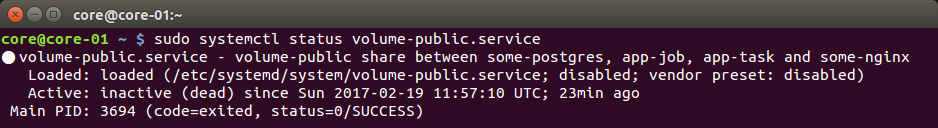
\includegraphics[width=0.85\textwidth]{images/figures/volume-public.service.png}
\caption{Estado de la unidad \kode{volume-public.service}.}
\end{figure}

\begin{figure}[H]
\centering
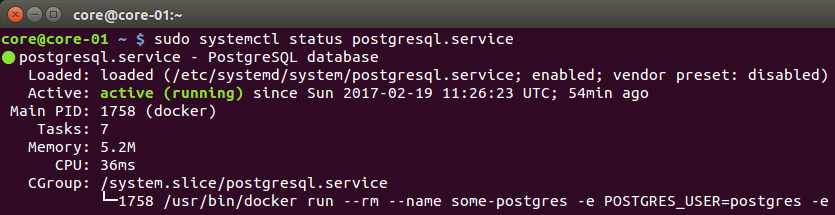
\includegraphics[width=0.8\textwidth]{images/figures/postgresql.service.png}
\caption{Estado de la unidad \kode{postgresql.service}.}
\end{figure}

\begin{figure}[H]
\centering
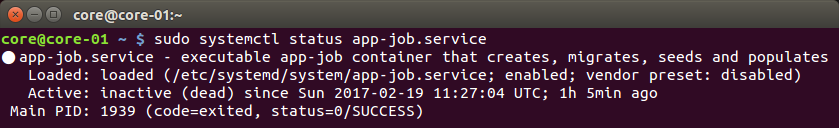
\includegraphics[width=0.8\textwidth]{images/figures/app-job.service.png}
\caption{Estado de la unidad \kode{app-job.service}.}
\end{figure}

\begin{figure}[H]
\centering
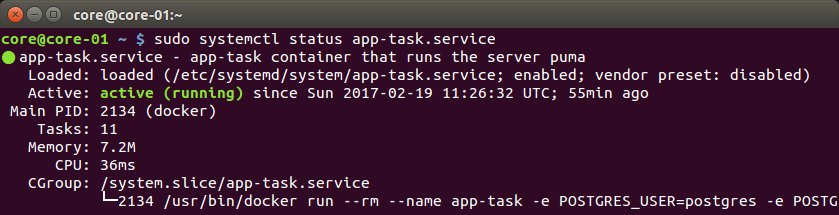
\includegraphics[width=0.8\textwidth]{images/figures/app-task.service.png}
\caption{Estado de la unidad \kode{app-task.service}.}
\end{figure}

\begin{figure}[H]
\centering
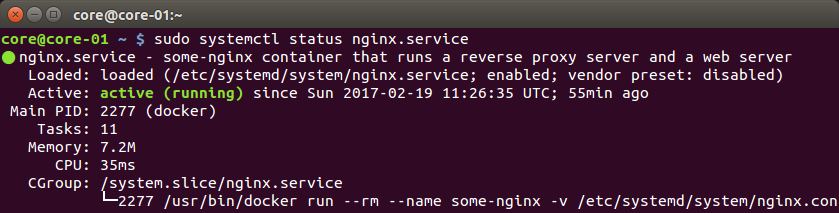
\includegraphics[width=0.8\textwidth]{images/figures/nginx.service.png}
\caption{Estado de la unidad \kode{nginx.service}.}
\end{figure}

Finalmente, se accede a la aplicación desde la máquina CoreOS y desde el sistema anfitrión:

\begin{figure}[H]
\centering
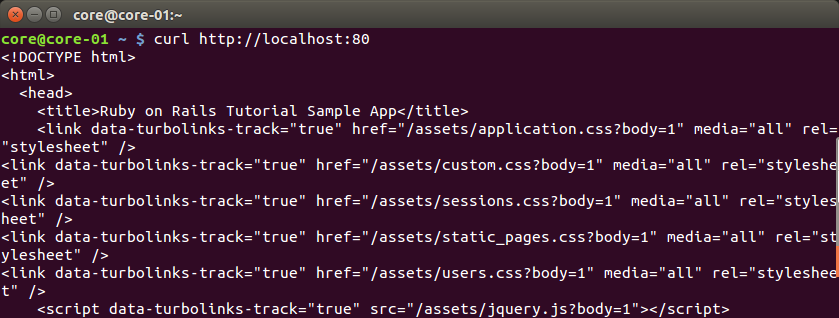
\includegraphics[width=0.7\textwidth]{images/figures/coreosmanualcurl.png}
\caption{Acceso a la aplicación desde la máquina CoreOS.}
\end{figure}

\begin{figure}[H]
\centering
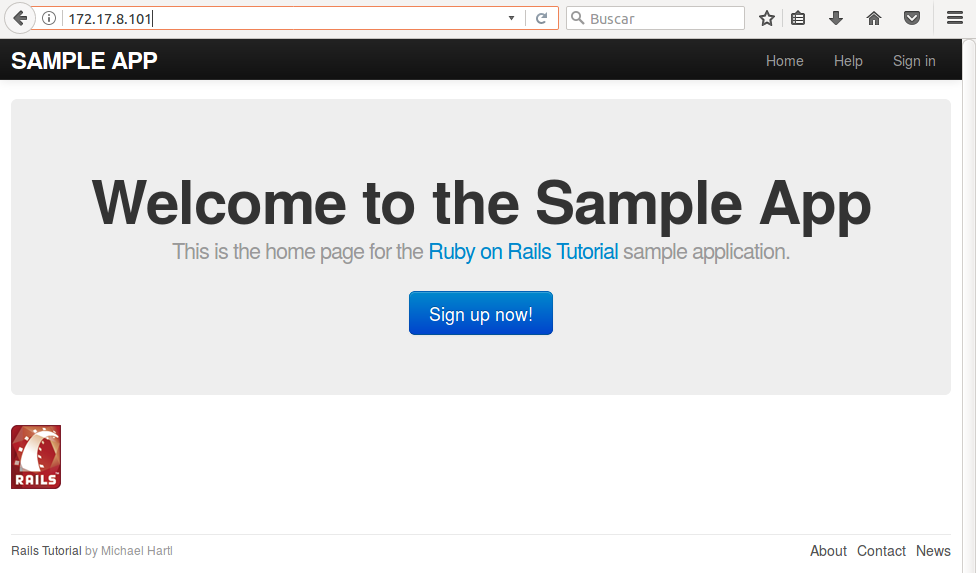
\includegraphics[width=0.7\textwidth]{images/figures/coreosmanualhost.png}
\caption{Acceso a la aplicación desde el sistema anfitrión.}
\end{figure}

\subsection{Despliegue automático de las unidades systemd}

Para realizar el despliegue de manera automática se hace uso del fichero \kode{cloud-config} denominado \kode{user-data.sampleapp.vbox}. Este fichero especifica el orden de las unidades a desplegar y las acciones de habilitación y comienzo de los servicios a los que hacen referencia.

Esta vez no se usará el almacenamiento NFS compartido por lo que ya no es necesaria la línea de provisión del \textit{script} en el fichero \kode{Vagranfile}. Además, puede volver a comentarse la línea que habilitaba este tipo de almacenamiento. De esta manera, también será necesario definir las variables de entorno, indicando la ruta, sus permisos y contenido. Lo mismo se realiza para el fichero que contiene la configuración Nginx.

Así, los añadidos al fichero \kode{user-data.sampleapp.vbox} son:

\begin{codelisting}
\label{code:vagrantfile2}
\codecaption{Fichero \kode{user-data.sampleapp.vbox}}
%= lang:yaml
\begin{code}
#cloud-config
---
write_files:
  - path: "/etc/postgres-credentials.env"
    permissions: "0644"
    content: |
      POSTGRES_USER=postgres
      POSTGRES_PASSWORD=postgres
  - path: "/etc/nginx.conf"
    permissions: "0644"
    content: |
      server {
        listen 80;
        root /usr/src/app/public;
        location / {
          proxy_set_header X-Forwarded-For $proxy_add_x_forwarded_for;
          proxy_set_header Host $http_host;
          proxy_redirect off;
          try_files $uri /page_cache/$uri /page_cache/$uri.html @app;
        }
        location @app{
          proxy_pass http://app:9292;
          break;
        }
      }
coreos:
  .
  units:
  .
  - name: volume-public.service
    command: start
    enable: true
    content: |
      [Unit] 
      Description= volume-public share between some-postgres, app-job, app-task
                   and some-nginx 
      After=docker.service
      Requires=docker.service
      [Service] 
      TimeoutStartSec=0 
      ExecStart=/usr/bin/docker volume create --name volume-public
      [Install] 
      WantedBy=multi-user.target
  - name: postgresql.service
    command: start
    enable: true
    content: |
      [Unit] 
      Description=PostgreSQL database 
      After=docker.service volume-public.service
      Requires=docker.service volume-public.service
      [Service] 
      TimeoutStartSec=0
      Restart=always
      EnvironmentFile=/etc/postgres-credentials.env
      ExecStartPre=-/usr/bin/docker kill some-postgres 
      ExecStartPre=-/usr/bin/docker rm some-postgres 
      ExecStartPre=/usr/bin/docker pull postgres 
      ExecStart=/usr/bin/docker run --rm --name some-postgres \
      -e "POSTGRES_USER=${POSTGRES_USER}" \
      -e "POSTGRES_PASSWORD=${POSTGRES_PASSWORD}" \
      -v "volume-public:/var/lib/postgresql" -p "5432:5432" postgres 
      ExecStop=/usr/bin/docker stop some-postgres
      [Install] 
      WantedBy=multi-user.target
  - name: app-job.service
    command: start
    enable: true
    content: |
      [Unit] 
      Description=executable app-job container that creates, migrates, seeds
                  and populates the database
      After=docker.service volume-public.service postgresql.service
      Requires=docker.service volume-public.service postgresql.service
      [Service] 
      TimeoutStartSec=0 
      EnvironmentFile=/etc/postgres-credentials.env
      ExecStartPre=-/usr/bin/docker kill app-job 
      ExecStartPre=-/usr/bin/docker rm app-job 
      ExecStartPre=/usr/bin/docker pull carolina/sample_app_rails_4_image:latest 
      ExecStart=/usr/bin/docker run --rm --name app-job \
                -v "volume-public:/usr/src/app/public" --entrypoint "./setup.sh" \
      -e "POSTGRES_USER=${POSTGRES_USER}" \
      -e "POSTGRES_PASSWORD=${POSTGRES_PASSWORD}" \
      -w "/usr/src/app" --link "some-postgres:db" \
      carolina/sample_app_rails_4_image:latest
      [Install] 
      WantedBy=multi-user.target
  - name: app-task.service
    command: start
    enable: true
    content: |
      [Unit] 
      Description=app-task container that runs the server puma
      After=docker.service volume-public.service postgresql.service 
            app-job.service
      Requires=docker.service volume-public.service postgresql.service 
               app-job.service
      [Service] 
      TimeoutStartSec=0
      Restart=always 
      EnvironmentFile=/etc/postgres-credentials.env
      ExecStartPre=-/usr/bin/docker kill app-task 
      ExecStartPre=-/usr/bin/docker rm app-task
      ExecStartPre=/usr/bin/docker pull carolina/sample_app_rails_4_image:latest 
      ExecStart=/usr/bin/docker run --rm --name app-task \
      -e "POSTGRES_USER=${POSTGRES_USER}" \
      -e "POSTGRES_PASSWORD=${POSTGRES_PASSWORD}" \
      -w "/usr/src/app" -v "volume-public:/usr/src/app/public" \
      --link "some-postgres:db" carolina/sample_app_rails_4_image:latest \
      /bin/bash -c "cp config/database.yml.postgresql \
      config/database.yml && cp ./.secret.example ./.secret && puma -p 9292"
      ExecStop=/usr/bin/docker stop app-task
      [Install] 
      WantedBy=multi-user.target
  - name: nginx.service
    command: start
    enable: true
    content: |
      [Unit] 
      Description=some-nginx container that runs a reverse proxy server and 
                  a web server
      After=docker.service volume-public.service postgresql.service 
            app-job.service app-task.service
      Requires=docker.service volume-public.service postgresql.service 
               app-job.service app-task.service
      [Service] 
      TimeoutStartSec=0
      Restart=always 
      ExecStartPre=-/usr/bin/docker kill some-nginx 
      ExecStartPre=-/usr/bin/docker rm some-nginx
      ExecStartPre=/usr/bin/docker pull nginx 
      ExecStart=/usr/bin/docker run --rm --name some-nginx \
      -v "/etc/nginx.conf:/etc/nginx/conf.d/default.conf" \
      -p "80:80" --link "app-task:app" \
      -v "volume-public:/usr/src/app/public" nginx 
      ExecStop=/usr/bin/docker stop some-nginx
      [Install] 
      WantedBy=multi-user.target
  \end{code}
\end{codelisting}

El fichero es validado con la utilidad \textit{Config Validator}\footnotettt{Config Validator}{https://coreos.com/validate}. 

\subsubsection{Despliegue de una instancia}

Con el despliegue se comprueba el correcto funcionamiento de la aplicación:

%= lang:bash
\begin{code}
$ vagrant up && vagrant ssh core-01
\end{code}

\subsection{Resultado}
Tanto si se decide realizar el despliegue manual o automático con unidades usando CoreOS se obtiene el correcto funcionamiento de la aplicación a través de cada servicio independiente.
El resultado en ambos casos ha sido positivo:

\begin{figure}[H]
\centering
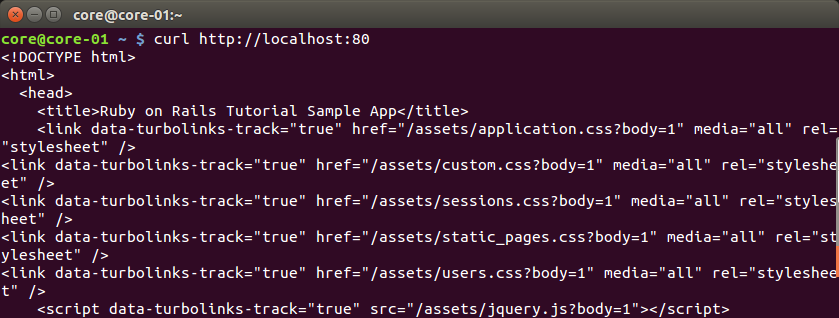
\includegraphics[width=0.7\textwidth]{images/figures/coreosmanualcurl.png}
\caption{Despliegue manual y automático. Acceso: máquina CoreOS.}
\end{figure}

\begin{figure}[H]
\centering
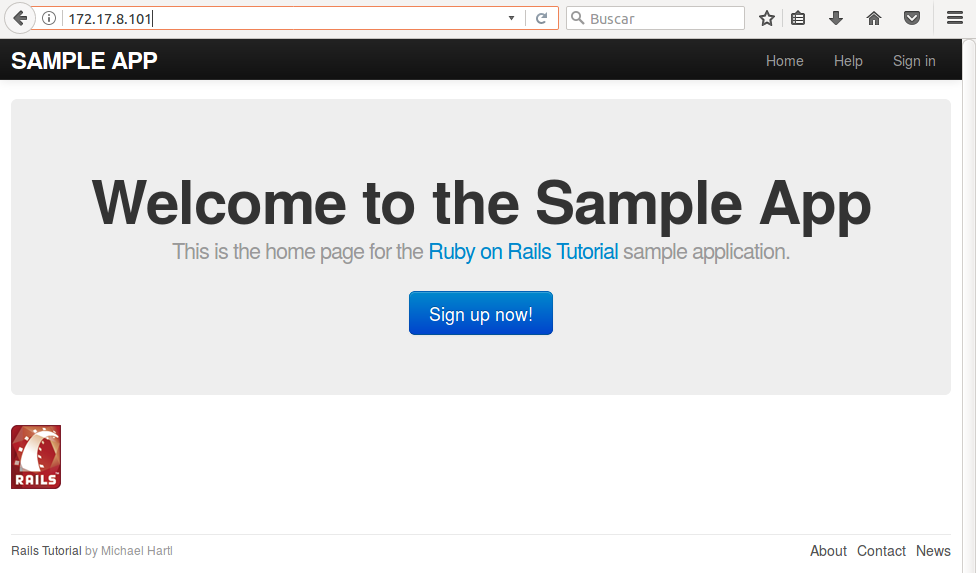
\includegraphics[width=0.7\textwidth]{images/figures/coreosmanualhost.png}
\caption{Despliegue manual y automático. Acceso: sistema anfitrión.}
\end{figure}

\section[Iteración 5: Despliegue en Amazon Web Services]{Iteración 5: Despliegue en la nube pública de Amazon Web Services}

En esta iteración se pretende desplegar la infraestructura en la nube pública de Amazon Web Services. Para ello se trabajará el mismo fichero \kode{config.rb}, el nuevo fichero \kode{user-data.sampleapp.aws} y el fichero \kode{Vagrantfile} en el que se introducirá el tratamiento e integración de este proveedor.

En la Figura \ref{fig:aws-1-iteration} puede distinguirse la distribución de las unidades de servicio, y por tanto, de los contenedores. El proxy, presente en el contenedor \kode{some-nginx}, que redirige al servidor web de la aplicación, en la máquina \kode{core-01}. Nginx será el servicio al cual los clientes y usuarios finales realizan las peticiones para acceder a la aplicación. No solo se va a tener un servidor de la aplicación, éste puede estar replicado desde en una a todas las instancias de la infraestructura y el servicio Nginx deberá balancear la carga entre ellos. Para controlar los servidores web que se registran y/o dejan de estar en el sistema se implementará un nuevo contenenedor, \kode{confd}, y un nuevo volumen Docker, \kode{conf-data}. A su vez, el contenedor \kode{some-postgres} para la base de datos se ubicará en la máquina \kode{core-02}. A él tiene que acceder tanto el contenedor \kode{app-job}, que la crea, migra y alimenta, como el contenedor \kode{app-task} que se dirige al mismo para obtener y escribir la información solicitada y añadida en la aplicación web. Ello se consigue con la implementación del contenedor \kode{skydns} que les servirá como servidor DNS, trabajando con las claves y valores de etc2.

\begin{figure}[H]
\centering
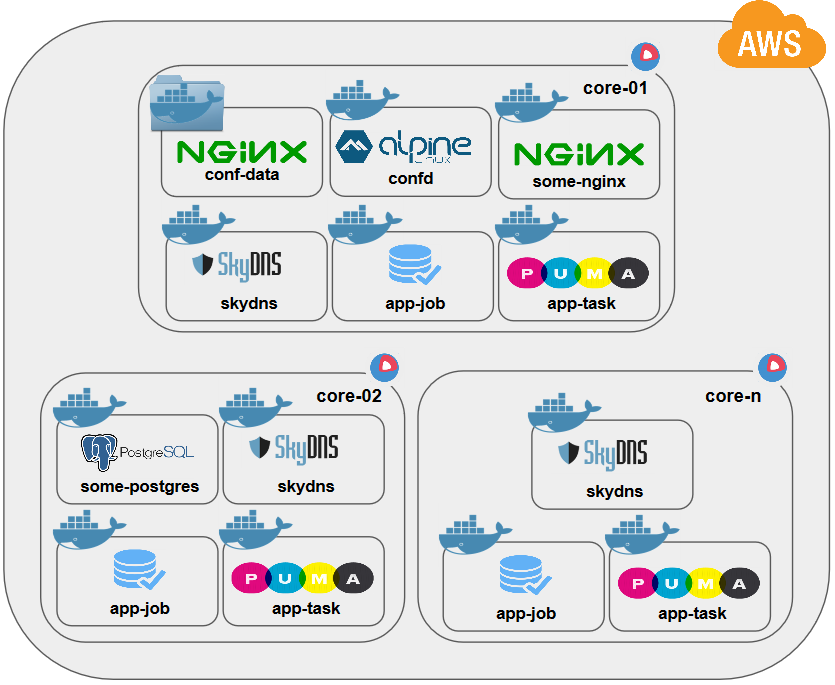
\includegraphics[width=0.7\textwidth]{images/figures/aws-1-iteration.png}
\caption{Distribución de la infraestructura a desplegar en AWS. \label{fig:aws-1-iteration}}
\label{fig:aws-1-iteration}
\end{figure}

La relación entre los contenedores, independientemente de su ubicación y replicación en otras instancias, en la manera en la que se ha comentado, puede apreciarse con mayor detalle en la Figura \ref{fig:aws-2-iteration}.

\begin{figure}[H]
\centering
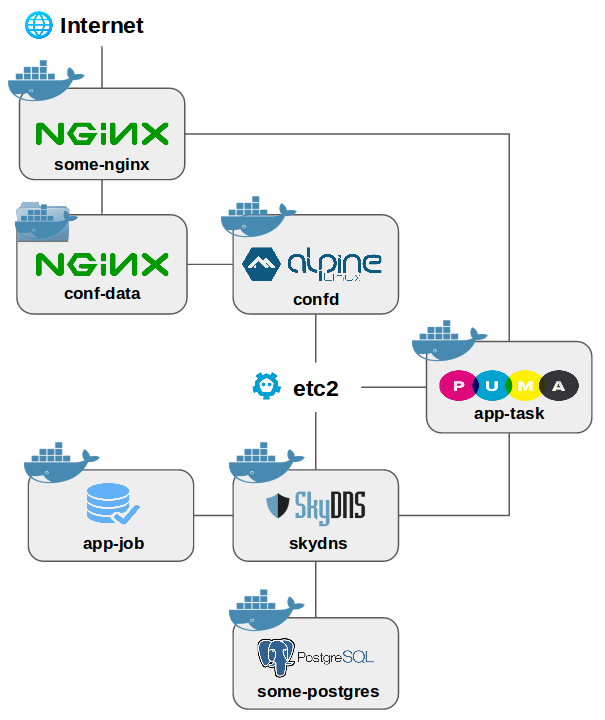
\includegraphics[width=0.5\textwidth]{images/figures/aws-2-iteration.png}
\caption{Relación entre los contenedores de la Infraestructura. \label{fig:aws-2-iteration}}
\end{figure}

Cuando la infraestructura se despliega, el contenedor \kode{some-postgres} se registra en \kode{skydns}, que utiliza etc2 para almacenar las claves y valores. De esta manera, \kode{some-postgres} puede ser descubierto por los contenedores \kode{app-job}, donde el primero en iniciarse creará, migrará y alimentará la base de datos. Cuando arrancan los contenedores \kode{app-task}, servidores web de la aplicación, se registran en etc2. El contenedor \kode{confd} vigila estos cambios cada 5 segundos para actualizar la configuración de \kode{some-nginx} y éste pueda resolver hacia ellos. Puesto que se comparte un fichero entre dos contenedores se utiliza el volumen \kode{conf-data}. Así, cuando un cliente realiza una petición a través de Internet a \kode{some-nginx}, éste puede redirigirle a uno de los servidores \kode{app-task}, el cuál consultará \kode{skydns} para poder obtener y escribir información en la base de datos. La política para redireccionar a los servidores web será \textit{Round Robin}, del primero al último.

Al ya no estar los contenedores en la misma instancia, compartir el volumen Docker \kode{volume-public} de la manera en la que se ha ido haciendo no es posible. Como no es el propósito directo su implementación se descontinúa y será incorporado en la sección de Trabajos Futuros \ref{trabajosfuturos}.

El servicio quedará disponible mediante el despliegue de la infraestructura desde Vagrant, estableciendo antes las variables de entorno correspondientes al proveedor. El acceso correcto al servicio puede ser probado desde la máquina \kode{core-01}, que contiene el proxy:

%= lang:bash
\begin{code}
$ . ~/.aws-credentials/aws-credentials
$ vagrant up --provider=aws
$ vagrant ssh core-01
# curl http://localhost:80
\end{code}

\begin{figure}[H]
\centering
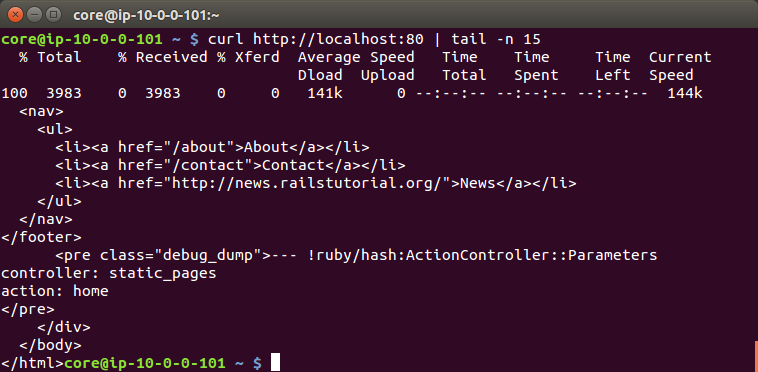
\includegraphics[width=0.65\textwidth]{images/figures/curl-confd.png}
\caption{Respuesta al servicio por comandos en \kode{core-01}.}
\end{figure}

\subsection{Obtención de la cuenta AWS}

Para la realización de esta iteración es necesario crear una cuenta en Amazon Web Services. En el caso presente se utilizará una cuenta que posee una capa gratuita, con una duración de un año, que se usa en conjunto con un crédito de \$50 dólares, proporcionado por dicha entidad. Este crédito ha sido facilitado al pertenecer al programa \textit{AWS Educate}\footnotettt{AWS Educate}{https://aws.amazon.com/es/grants/}. Se trata de una iniciativa de Amazon a nivel mundial que proporciona a los estudiantes y personal docente los recursos necesarios para acelerar el aprendizaje relacionado con la nube, así como para ayudar a formar a futuros empresarios e investigadores.

Los servicios de AWS se localizan en múltiples ubicaciones por todo el mundo. Tienen diferentes regiones y, en cada una de ellas, distintas zonas de disponibilidad. En este trabajo se escogerá la región \textit{US East} y zona \textit{N. Virginia}.

Se hace uso del servicio AWS \textit{Identity and Access Management} (IAM) con la intención de controlar de forma segura el acceso a servicios y recursos. Con el objetivo de tener un usuario para realizar las actividades de desarrollo, el primer paso será la creación del grupo \textit{deployers} con permiso para manejar las instancias EC2. Luego, se crea el usuario \textit{deployer} con tipo de acceso \textit{Management Console access}. Al mismo se le facilita una contraseña y se le indica que pertenece al grupo recién creado.

\subsection{Creación de la red y subred virtual}

El servicio \textit{Virtual Private Cloud} (VPC) permite controlar todos los aspectos del entorno de red virtual. Será usado con la intención de hacer la selección del rango de direcciones IP que se les dará a las máquinas virtuales y para crear una subred acorde.

En primer lugar se crea una VPC llamada \textit{vpc-sampleapp} con el rango de direcciones IPv4 10.0.0.0/16:

\begin{figure}[H]
\centering
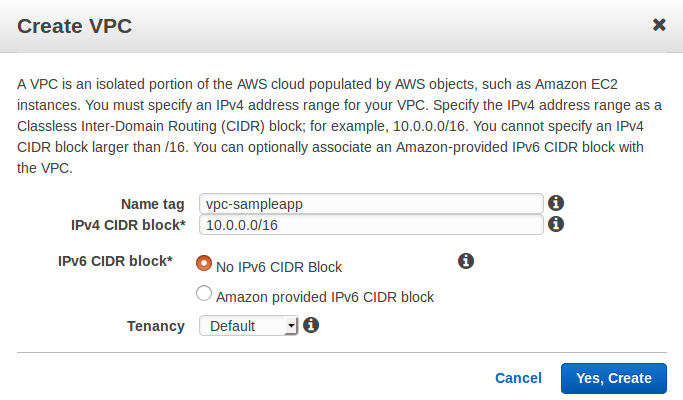
\includegraphics[width=0.7\textwidth]{images/figures/vpc-sampleapp.png}
\caption{Creación de la VPC \textit{vpc-sampleapp}.}
\end{figure}

En segundo lugar se crea una subred llamada \textit{subnet-sampleapp}, perteneciente a la anterior VPC, con el rango de direcciones IPv4 10.0.0.0/24:

\begin{figure}[H]
\centering
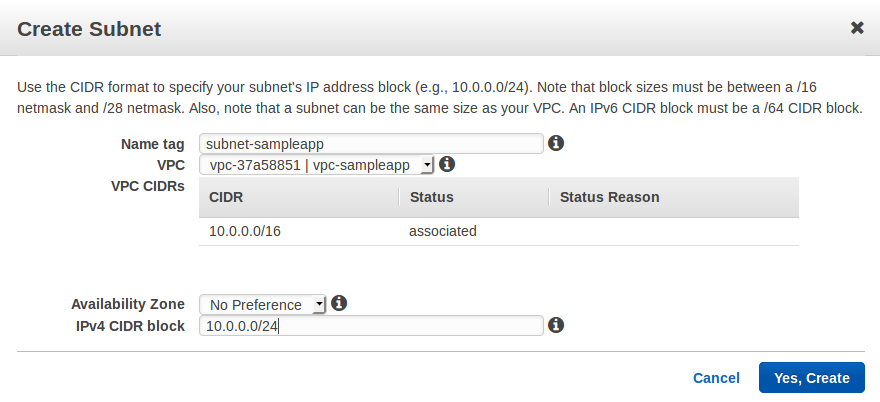
\includegraphics[width=0.8\textwidth]{images/figures/subnet-sampleapp.png}
\caption{Creación de la subred \textit{subnet-sampleapp}.}
\end{figure}

\subsection{Creación del par de claves y del grupo de seguridad}

Lo siguiente es preparar una pareja de claves \textit{key pair} para poder entrar por SSH en la instancia lanzada. Para ello es necesario crear un \textit{Security Group} que defina los puertos de entrada por los que podrá recibir peticiones.

Lo primero se realiza accediendo al servicio Amazon Elastic Cloud Computing (Amazon EC2) y navegando hasta \textit{Network \& Security, Key Pairs}. Aquí, se crea una nueva pareja de claves con el nombre \kode{keypair.pem}, la cual se guarda en un directorio oculto de nombre \kode{\textasciitilde{}/.aws-credentials}, facilitando permisos de lectura y escritura al propietario:

%= lang:bash
\begin{code}
$ mkdir ~/.aws-credentials
$ mv /home/carolina/Descargas/keypair.pem ~/.aws-credentials/
$ chmod 0600 ~/.aws-credentials/keypair.pem
\end{code}

Ahora se navega hasta \textit{Network \& Security, Security Groups} y se crea el grupo de seguridad \textit{deploying-security-group} con las reglas TCP entrantes que permitan dejar pasar a la instancia las peticiones que llegan para conexiones a los puertos asignados a los protocolos SSH (22) y HTTP (80). También se añaden las reglas TCP a los puertos que utiliza CoreOS en sus comunicaciones con los clientes, siendo 2379, 2380, 4001 y 7001. Con la intención de que, en un momento dado, las distintas máquinas virtuales que se creen, formando un clúster CoreOS, tengan conectividad con los contenedores de otras máquinas virtuales miembro se habilita el puerto 8285 mediante una regla UDP. Finalmente, se añaden las reglas TCP sobre los puertos que afectan a la aplicación, 9292 para el servidor puma y 5432 para el servidor PostgreSQL.

\subsection{Configuración del fichero user-data}

Para llevar a cabo esta parte se necesita una nueva configuración \kode{cloud-config}. Este nuevo \kode{user-data} recibirá el nombre de \kode{user-data.sampleapp.aws}. Tendrá, únicamente, dos diferencias respecto al anterior, por ello se copia:

%= lang:bash
\begin{code}
$ cp user-data.sampleapp.vbox user-data.sampleapp.aws
\end{code}

La primera de las diferencias será especificar al servicio flannel que ha de usar el rango de direcciones IPv4 privadas, pues los contenedores internos a la máquina usarán una red privada para no ser accesibles desde el exterior. El segundo cambio detalla que la red privada a usar será la 172.17.0.0/16 y el protocolo UDP.

\begin{codelisting}
\label{code:vagrantfile2}
\codecaption{Fichero \kode{user-data.sampleapp.aws}}
%= lang:yaml
\begin{code}
.
coreos:
  .
  flannel:
    interface: "$private_ipv4"
  units:
  .
  - name: flanneld.service
    drop-ins:
    - name: 50-network-config.conf
      content: |
        [Service]
        ExecStartPre=/usr/bin/etcdctl set /coreos.com/network/config 
               '{ "Network": "172.17.0.0/16", "Backend": { "Type": "udp" } }'
.
\end{code}
\end{codelisting}

\subsection{Configuración del fichero Vagrantfile}

Primero se instala el plugin necesario para utilizar AWS como proveedor:

%= lang:bash
\begin{code}
$ vagrant plugin install vagrant-aws
\end{code}

Luego se añade al fichero \kode{Vagrantfile} la comprobación de que se encuentre instalado en el sistema anfitrión.

Para poder iniciar sesión en la cuenta AWS como usuario \textit{deployer} se agregará un fichero local en el que especificar estos datos sensibles, con la intención de ser tratados como variables de entorno. Para ello se crea el fichero \kode{\textasciitilde{}/.aws-credentials/aws-credentials} con permiso de ejecución \textit{chmod +x} y contenido:

\begin{codelisting}
\label{code:vagrantfile2}
\codecaption{Fichero \kode{\textasciitilde{}/.aws-credentials/aws-credentials}}
%= lang:bash
\begin{code}
export AWS_KEY='XXXXXXXXXXXXXXXXXXX'
export AWS_SECRET='XXXXXXXXXXXXXXXXXXXXXXXXXXX'
export AWS_KEYNAME='keypair'
export AWS_KEYPATH='~/.aws-credentials/keypair.pem'
\end{code}
\end{codelisting}

Así, en el propio \kode{Vagrantfile} se especificará que las variables de entorno \kode{ENV['AWS\_KEY']}, \kode{ENV['AWS\_SECRET']} y \kode{ENV['AWS\_KEYNAME']} deben establecerse para continuar. Para ello se ejecuta en el directorio actual:

%= lang:bash
\begin{code}
$ . ~/.aws-credentials/aws-credentials
\end{code}

Luego, como en el caso anterior, se prepara la copia del fichero \kode{cloud-config} de \kode{user-data.sampleapp.aws} a \kode{user-data}.

Todas las opciones necesarias para el despliegue desde Vagrant con este proveedor vienen a determinar la configuración de la instancia o instancias a lanzar. Las características que interesan definir son las siguientes:
\begin{itemize}
\item \textit{access\_key\_id}: Primera clave, perteneciente al identificador del usuario.
\item \textit{secret\_access\_key}: Segunda clave, perteneciente a la contraseña secreta.
\item \textit{keypair\_name}: Nombre del archivo que contiene el par de claves.
\item \textit{aws\_region}: Región.
\item \textit{aws\_availability\_zone}: Zona de disponibilidad.
\item \textit{aws\_subnet\_id}: Identificador de la subred.
\item \textit{aws\_security\_groups}: Identificador del grupo de seguridad.
\item \textit{aws\_ami}: Identificador de la \textit{Amazon Machine Image} (AMI). Se escoge \textit{CoreOS-alpha-1339.0.0-hvm - ami-00598116}, de 64 bits con el tipo de virtualización HVM.
\item \textit{aws\_instance\_type}: Tipo de instancia a lanzar. El tipo será \textit{t2.micro Free tier eligible}.
\item \textit{aws\_elastic\_ip}: Indicación de uso de direcciones IP elásticas para el acceso remoto al servicio.
\item \textit{private\_ip\_adresses}: Dirección IP privada a asignar a la instancia.
\item \textit{user\_data}: Contenido del fichero \kode{user-data}.
\end{itemize}

Los valores que tomarán estos parámetros son los relativos a las diferentes creaciones que se han ido realizando con la cuenta en uso.

Otro aspecto a indicar es la deshabilitación de la carpeta compartida por defecto \kode{/vagrant} con el directorio actual del sistema anfitrión, pues es prescindible para el despliegue del servicio. También será necesario indicar la \textit{url} que utilizará Vagrant como \textit{box}, imagen para la máquina virtual. Dicha indicación ha de ir acompañada del nombre de usuario, ruta del fichero del par de claves y la opción de que no se desea clave para iniciar sesión. Todo ello especificado al protocolo SSH (22), usado para conectarse con la instancia.

Finalmente solo queda copiar el fichero \kode{cloud-config} a la instancia. Aquí se ha optado por crear una copia del fichero \kode{user-data} por máquina, identificándola con un número. El contenido del fichero original será copiado al segundo mediante métodos propios a \kode{YAML}. Una vez hecha la copia, se indica la dirección IP que la máquina va adquirir, siendo 10.0.0.10X, y se pasa el contenido mediante su lectura, haciendo uso del campo \kode{user\_data}.

Así, al fichero \kode{Vagrantfile} se le añade lo siguiente:

\begin{codelisting}
\label{code:vagrantfile2}
\codecaption{Fichero \kode{Vagrantfile}}
%= lang:bash
\begin{code}
.
if (!ARGV.nil? && ARGV.join('').include?('provider=aws'))
  unless Vagrant.has_plugin?("vagrant-aws") 
    abort("Did not detect vagrant-aws plugin... 
           vagrant plugin install vagrant-aws")
  end
  unless ENV['AWS_KEY'] && ENV['AWS_SECRET'] && ENV['AWS_KEYNAME']
    abort("$AWS_KEY && $AWS_SECRET && $AWS_KEYNAME should set before...")
  end
  FileUtils.cp_r(File.join(File.dirname(__FILE__), "user-data.sampleapp.aws"), 
  File.join(File.dirname(__FILE__), "user-data"), :remove_destination => true)
end
.
$aws_region = 'us-east-1'
$aws_availability_zone = 'us-east-1a'
$aws_subnet_id = 'subnet-b17d79ea'
$aws_security_groups = 'sg-3319964c'
$aws_ami = 'ami-00598116'
$aws_instance_type = 't2.micro'
$aws_elastic_ip = true
.
Vagrant.configure("2") do |config|
 .
  config.vm.provider :aws do |aws, override|
    aws.access_key_id = ENV['AWS_KEY']
    aws.secret_access_key = ENV['AWS_SECRET']
    aws.keypair_name = ENV['AWS_KEYNAME']
    aws.security_groups = $aws_security_groups
    aws.ami = $aws_ami
    aws.instance_type = $aws_instance_type
    aws.region = $aws_region
    aws.subnet_id = $aws_subnet_id
    aws.elastic_ip = $aws_elastic_ip
    override.vm.synced_folder ".", "/vagrant", disabled: true
    override.ssh.username = "core"
    override.ssh.private_key_path = ENV['AWS_KEYPATH']
    override.ssh.insert_key = false
    override.vm.box_url = "https://github.com/mitchellh/vagrant-aws/raw/master/
                           dummy.box"
  end
  .
  (1..$num_instances).each do |i|
    config.vm.define vm_name = "%s-%02d" % [$instance_name_prefix, i] do |config|
      .
      if File.exist?(CLOUD_CONFIG_PATH) && ARGV[0].eql?('up')
        .
        config.vm.provider :aws do |aws, override|   
          user_data_specific = "#{CLOUD_CONFIG_PATH}-#{i}"
          require 'yaml'
          data = YAML.load(IO.readlines(CLOUD_CONFIG_PATH)[1..-1].join)
          yaml = YAML.dump(data)
          File.open(user_data_specific, 'w') do |file|
            file.write("#cloud-config\n\n#{yaml}")
          end
          aws.private_ip_address = "10.0.0.#{100+i}"
          aws.user_data = File.read(user_data_specific)
        end
      end
    end
  end
end
\end{code}
\end{codelisting}

\subsection{Despliegue de una instancia}

A continuación se despliega esta infraestructura y se accede a la instancia:

%= lang:bash
\begin{code}
$ vagrant up --provider=aws && vagrant ssh core-01
\end{code}

Ahora se prueba que la salud del clúster es positiva:

%= lang:bash
\begin{code}
# etcdctl cluster-health
\end{code}

\begin{figure}[H]
\centering
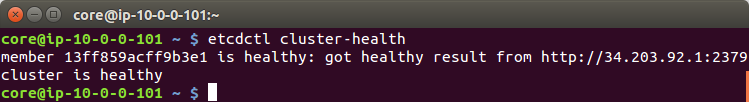
\includegraphics[width=0.7\textwidth]{images/figures/cluster-health-aws-1.png}
\caption{Comprobación de la salud del clúster con 1 instancia.}
\end{figure}

Además se comprueba que la red virtual funciona correctamente:

%= lang:bash
\begin{code}
$ sudo systemctl status flanneld
\end{code}

\begin{figure}[H]
\centering
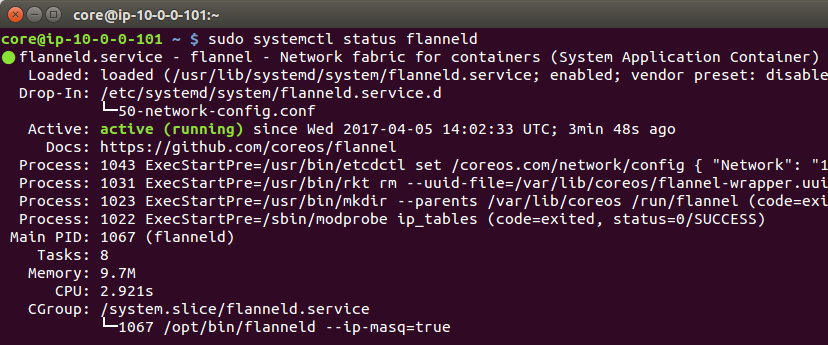
\includegraphics[width=0.7\textwidth]{images/figures/flanneld-aws-1.png}
\caption{Comprobación de la red virtual - \kode{core01}.}
\end{figure}

Por último se comprueba desde la consola de comandos que se puede acceder al servicio correctamente con el comando \kode{curl}:

%= lang:bash
\begin{code}
$ curl http://localhost:80 | tail -n 15
\end{code}

\begin{figure}[H]
\centering
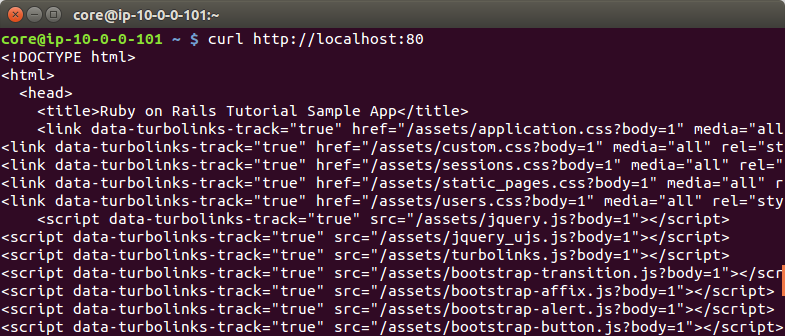
\includegraphics[width=0.7\textwidth]{images/figures/curl-aws-1.png}
\caption{Acceso al servicio desde la máquina \kode{core01}.}
\end{figure}

Además, se utiliza la IP elástica para acceder a través del navegador web:

\begin{figure}[H]
\centering
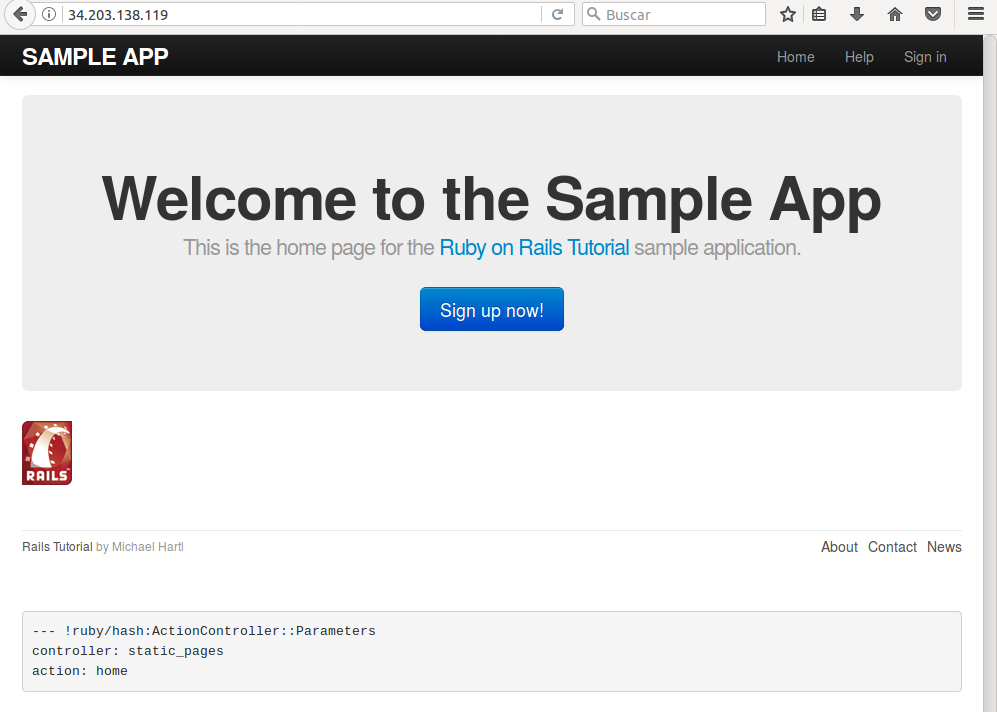
\includegraphics[width=0.7\textwidth]{images/figures/access-aws-1.png}
\caption{Acceso al servicio desde el sistema anfitrión.}
\end{figure}

Desde la consola de AWS se puede apreciar dicha instancia:

\begin{figure}[H]
\image{images/figures/aws-console-1.png}
\caption{Máquina \kode{core-01} desde la consola de AWS.}
\end{figure}

Para destruir la infraestructura y los recursos asociados a ella, se ejecuta lo siguiente:

%= lang:bash
\begin{code}
$ vagrant destroy -f
\end{code}

\subsection{Despliegue de tres instancias}

Para realizar el despliegue de un clúster con varias máquinas virtuales se cambia el valor de la variable \kode{num\_instances} a 3 en los ficheros \kode{Vagrantfile} y \kode{config.rb}. De esta manera se tiene en cada una de las instancias una copia del mismo servicio.

A continuación se despliega esta infraestructura:

%= lang:bash
\begin{code}
$ vagrant up --provider=aws
\end{code}

Se prueba, desde el sistema anfitrión, que la salud del clúster es positiva en todas las máquinas:

%= lang:bash
\begin{code}
$ for i in 1 2 3; do vagrant ssh core-0$i -c 'etcdctl cluster-health'; done
\end{code}

\begin{figure}[H]
\centering
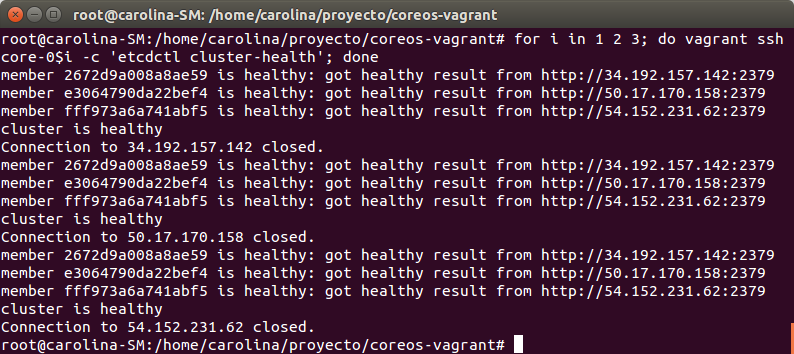
\includegraphics[width=0.7\textwidth]{images/figures/cluster-health-aws-3.png}
\caption{Comprobación de la salud del clúster.}
\end{figure}

Además, se comprueba que la red virtual funciona correctamente:

%= lang:bash
\begin{code}
$ for i in 1 2 3; do vagrant ssh core-0$i -c 'sudo systemctl flanneld \
  | head -n16'; done
\end{code}

\begin{figure}[H]
\centering
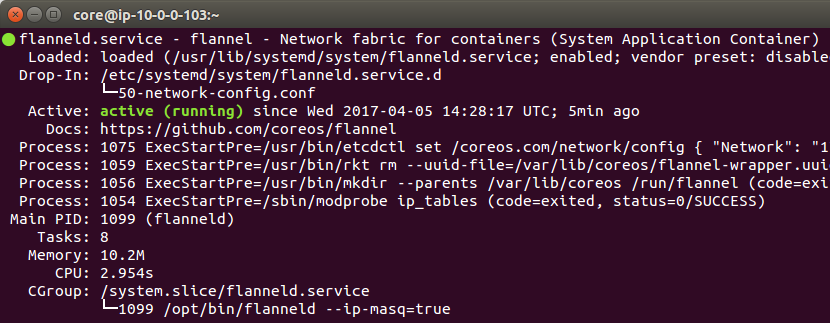
\includegraphics[width=0.8\textwidth]{images/figures/flanneld-aws-3.png}
\caption{Comprobación de la red virtual.}
\end{figure}

Para probar que las máquinas virtuales tienen conexión con los contenedores de otras máquinas virtuales se obtiene, en primer lugar, la dirección IP del contenedor \kode{some-postgres} de la máquina virtual \kode{core-03}:

%= lang:bash
\begin{code}
# docker inspect some-postgres
\end{code}

\begin{figure}[H]
\centering
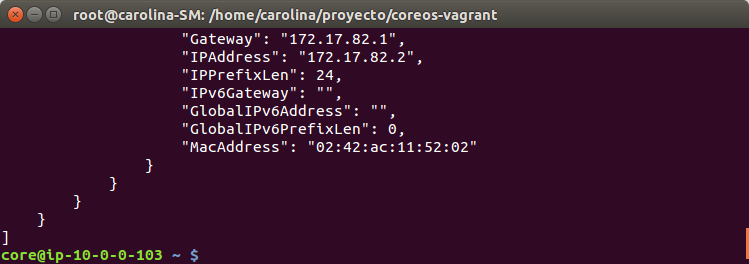
\includegraphics[width=0.8\textwidth]{images/figures/docker-inspect-3.png}
\caption{Obtención de la dirección IP de un contenedor en \kode{core-03}.}
\end{figure}

Luego se prueba que haya conexión desde la máquina virtual \kode{core-01}:

%= lang:bash
\begin{code}
# ping 172.17.82.2
\end{code}

\begin{figure}[H]
\centering
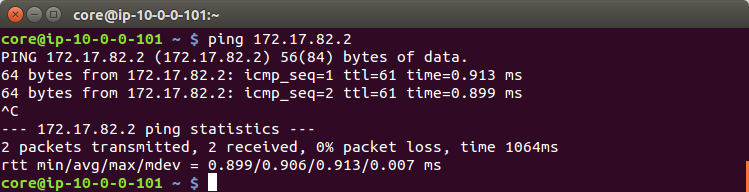
\includegraphics[width=0.8\textwidth]{images/figures/ping-1.png}
\caption{Prueba de conexión a un contenedor de \kode{core-03} desde \kode{core-01}.}
\end{figure}

Por último se comprueba que se puede acceder al servicio desde la consola de comandos, con el comando \kode{curl}, y desde el navegador web, con la dirección IP elástica. Desde la consola de AWS se podrán observar las instancias  

%= lang:bash
\begin{code}
$ for i in 1 2 3; do vagrant ssh core-0$i -c 'curl http://localhost:80 \
  | tail -n 15'; done
\end{code}

\begin{figure}[H]
\centering
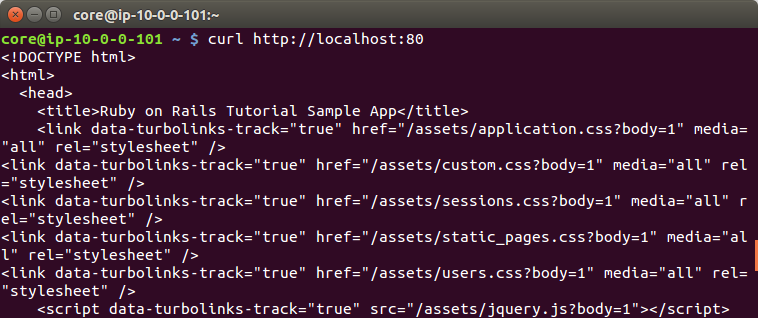
\includegraphics[width=0.8\textwidth]{images/figures/curl-aws-3.png}
\caption{Acceso al servicio por consola de comandos.}
\end{figure}

\begin{figure}[H]
\centering
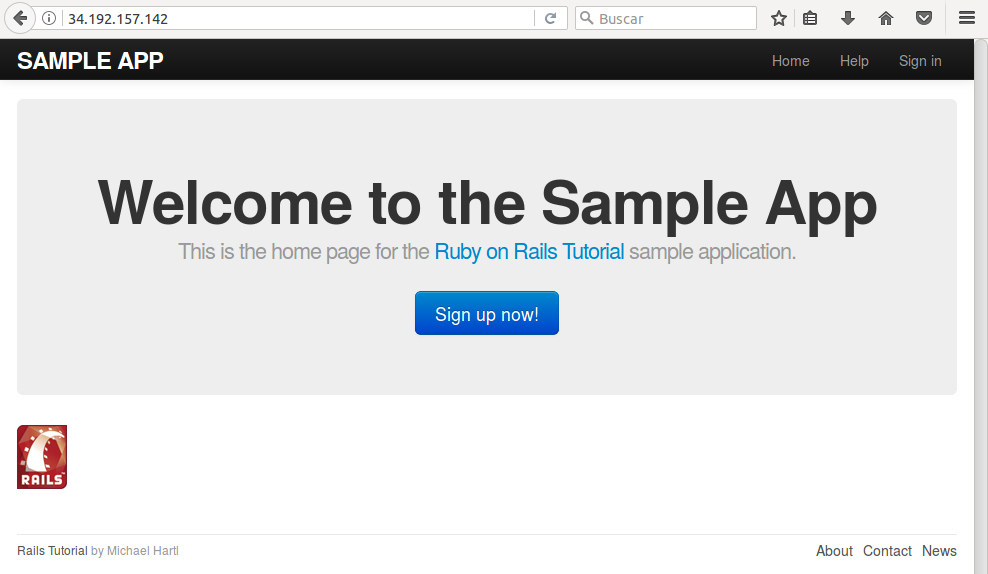
\includegraphics[width=0.65\textwidth]{images/figures/nav-1.png}
\caption{Acceso al servicio por el navegador web desde \kode{core-01}.}
\end{figure}

\begin{figure}[H]
\centering
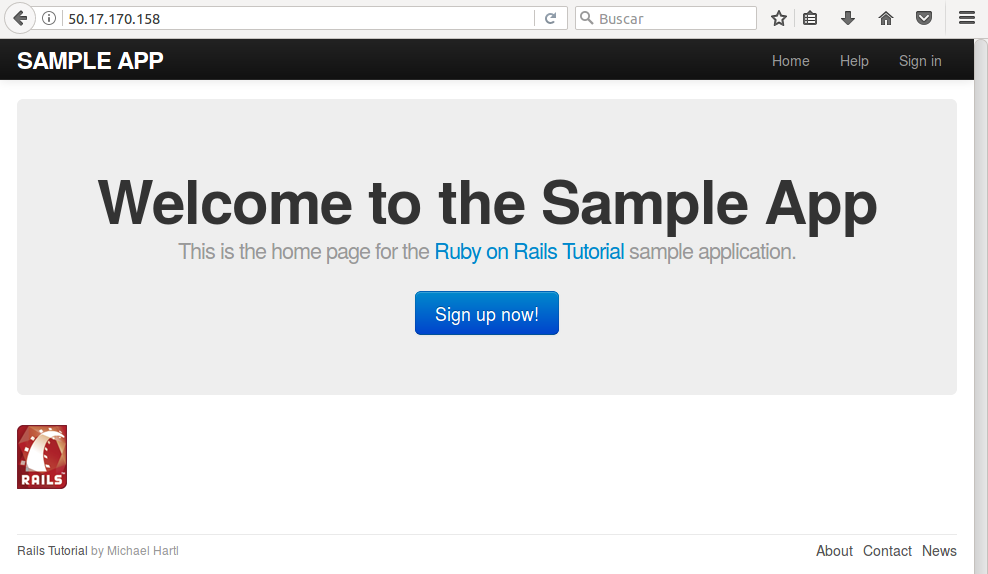
\includegraphics[width=0.65\textwidth]{images/figures/nav-2.png}
\caption{Acceso al servicio por el navegador web desde \kode{core-02}.}
\end{figure}

\begin{figure}[H]
\centering
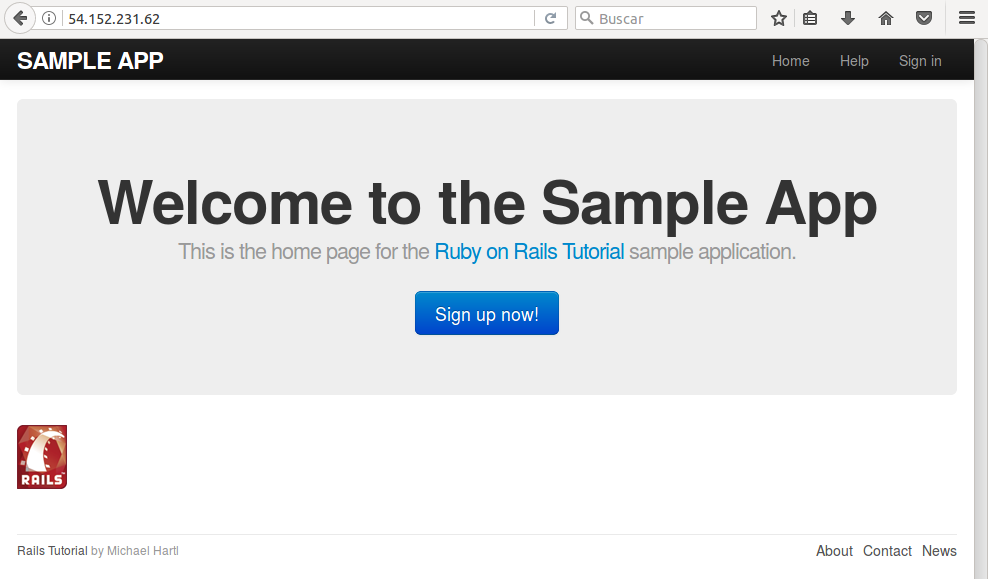
\includegraphics[width=0.65\textwidth]{images/figures/nav-3.png}
\caption{Acceso al servicio por el navegador web desde \kode{core-03}.}
\end{figure}

\begin{figure}[H]
\centering
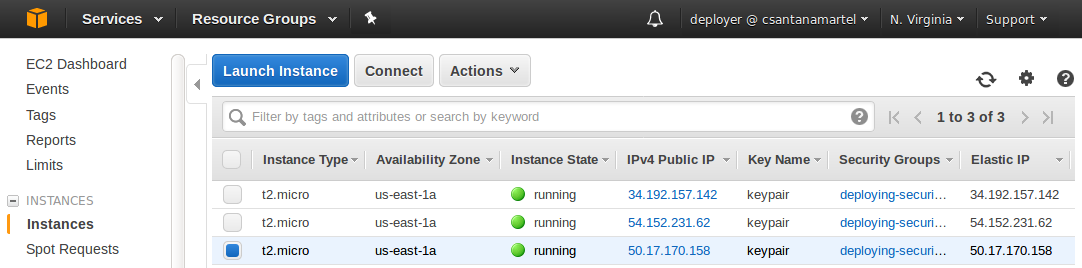
\includegraphics[width=0.95\textwidth]{images/figures/aws-console-3.png}
\caption{Consola AWS EC2 Instances - \kode{core-01}, \kode{core-02} y \kode{core-03}.}
\end{figure}

\subsection{Cambio de las unidades systemd a fleet}

Hasta ahora las unidades de servicio se han configurado globalmente en la sección propia de systemd. Con la intención de mejorar la distribución de la infraestructura se va a pasar a tratar a las unidades de servicio \kode{volume-public.service}, \kode{postgresql.service}, \kode{app-job.service}, \kode{app-task.service} y \kode{nginx.service} como unidades fleet. Para ello es necesario que los servicios sean especificados como ficheros a escribir en el sistema, concretamente se van a situar en la ruta \kode{/home/core/}. La sección \kode{[Install]} se cambia por la propia a fleet, \kode{[X-Fleet]}. Aquí se especificará el parámetro \kode{Global} que programa la unidad en todos los agentes del clúster de forma que desde cada una de las instancias que lo componen se puedan ver todos los servicios que hay en ellas. Luego se crean como unidades de servicio systemd los servicios empezados por \kode{fleet-}, para cada uno de ellos, que se van a encargar de indicar a fleet que ha de empezar los servicios pasados como ficheros. 

De esta manera, continuando con el clúster de 3 instancias, se realizan las siguientes modificaciones en el fichero \kode{user-data.sampleapp-aws}:

\begin{codelisting}
\label{code:vagrantfile2}
\codecaption{Fichero \kode{user-data.sampleapp-aws}}
%= lang:yaml
\begin{code}
#cloud-config
---
write_files:
  .
  - path: "/home/core/volume-public.service"
    permissions: "0644"
    content: |
      [Unit] 
      Description= volume-public share between some-postgres, app-job, app-task 
                   and some-nginx 
      After=docker.service
      Requires=docker.service
      [Service] 
      TimeoutStartSec=0 
      ExecStart=/usr/bin/docker volume create --name volume-public
      [X-Fleet]
      Global=true
  - path: "/home/core/postgresql.service"
    permissions: "0644"
    content: |
      [Unit] 
      Description=PostgreSQL database 
      After=docker.service volume-public.service
      Requires=docker.service volume-public.service
      [Service] 
      TimeoutStartSec=0
      Restart=always
      EnvironmentFile=/etc/postgres-credentials.env
      ExecStartPre=-/usr/bin/docker kill some-postgres 
      ExecStartPre=-/usr/bin/docker rm some-postgres 
      ExecStartPre=/usr/bin/docker pull postgres 
      ExecStart=/usr/bin/docker run --rm --name some-postgres \
      -e "POSTGRES_USER=${POSTGRES_USER}" \
      -e "POSTGRES_PASSWORD=${POSTGRES_PASSWORD}" \
      -v "volume-public:/var/lib/postgresql" -p "5432:5432" postgres 
      ExecStop=/usr/bin/docker stop some-postgres
      [X-Fleet]
      Global=true
  - path: "/home/core/app-job.service"
    permissions: "0644"
    content: |
      [Unit] 
      Description=executable app-job container that creates, migrates, seeds and 
                  populates the database
      After=docker.service volume-public.service postgresql.service
      Requires=docker.service volume-public.service postgresql.service
      [Service] 
      TimeoutStartSec=0 
      EnvironmentFile=/etc/postgres-credentials.env
      ExecStartPre=-/usr/bin/docker kill app-job 
      ExecStartPre=-/usr/bin/docker rm app-job 
      ExecStartPre=/usr/bin/docker pull carolina/sample_app_rails_4_image:latest 
      ExecStart=/usr/bin/docker run --rm --name app-job \
      -v "volume-public:/usr/src/app/public" --entrypoint "./setup.sh" \
      -e "POSTGRES_USER=${POSTGRES_USER}" \
      -e "POSTGRES_PASSWORD=${POSTGRES_PASSWORD}" \
      -w "/usr/src/app" --link "some-postgres:db" \
      carolina/sample_app_rails_4_image:latest
      [X-Fleet]
      Global=true
  - path: "/home/core/app-task.service"
    permissions: "0644"
    content: |
      [Unit] 
      Description=app-task container that runs the server puma
      After=docker.service volume-public.service postgresql.service 
            app-job.service
      Requires=docker.service volume-public.service postgresql.service 
               app-job.service
      [Service] 
      TimeoutStartSec=0
      Restart=always 
      EnvironmentFile=/etc/postgres-credentials.env
      ExecStartPre=-/usr/bin/docker kill app-task 
      ExecStartPre=-/usr/bin/docker rm app-task
      ExecStartPre=/usr/bin/docker pull carolina/sample_app_rails_4_image:latest 
      ExecStart=/usr/bin/docker run --rm --name app-task \
      -e "POSTGRES_USER=${POSTGRES_USER}" \
      -e "POSTGRES_PASSWORD=${POSTGRES_PASSWORD}" \
      -w "/usr/src/app" -v "volume-public:/usr/src/app/public" \
      --link "some-postgres:db" \
      carolina/sample_app_rails_4_image:latest \
      /bin/bash -c "cp config/database.yml.postgresql config/database.yml && \
      cp ./.secret.example ./.secret && puma -p 9292"
      ExecStop=/usr/bin/docker stop app-task
      [X-Fleet]
      Global=true
  - path: "/home/core/nginx.service"
    permissions: "0644"
    content: |
      [Unit] 
      Description=some-nginx container that runs a reverse proxy server and a 
                  web server
      After=docker.service volume-public.service postgresql.service 
            app-job.service app-task.service
      Requires=docker.service volume-public.service postgresql.service 
               app-job.service app-task.service
      [Service] 
      TimeoutStartSec=0
      Restart=always 
      ExecStartPre=-/usr/bin/docker kill some-nginx 
      ExecStartPre=-/usr/bin/docker rm some-nginx
      ExecStartPre=/usr/bin/docker pull nginx 
      ExecStart=/usr/bin/docker run --rm --name some-nginx \
      -v "/etc/nginx.conf:/etc/nginx/conf.d/default.conf" \
      -p "80:80" --link "app-task:app" \
      -v "volume-public:/usr/src/app/public" nginx 
      ExecStop=/usr/bin/docker stop some-nginx
      [X-Fleet]
      Global=true
coreos:
  .
  units:
  .
  - name: fleet-volume-public.service
    command: start
    content: |
      [Unit]
      Description=Start volume-public.service using fleet
      [Service]
      ExecStart=/usr/bin/fleetctl start /home/core/volume-public.service
  - name: fleet-postgresql.service
    command: start
    content: |
      [Unit]
      Description=Start postgresql.service using fleet
      [Service]
      ExecStart=/usr/bin/fleetctl start /home/core/postgresql.service
  - name: fleet-app-job.service
    command: start
    content: |
      [Unit]
      Description=Start app-job.service using fleet
      [Service]
      ExecStart=/usr/bin/fleetctl start /home/core/app-job.service
  - name: fleet-app-task.service
    command: start
    content: |
      [Unit]
      Description=Start app-task.service using fleet
      [Service]
      ExecStart=/usr/bin/fleetctl start /home/core/app-task.service
  - name: fleet-nginx.service
    command: start
    content: |
      [Unit]
      Description=Start nginx.service using fleet
      [Service]
      ExecStart=/usr/bin/fleetctl start /home/core/nginx.service
\end{code}
\end{codelisting}

Para comprobar que funciona se levanta la infraestructura:

%= lang:bash
\begin{code}
$ vagrant up --provider=aws
\end{code}

\begin{figure}[H]
\image{images/figures/aws-console-fleet.png}
\caption{Consola AWS EC2 Instances - \kode{core-01}, \kode{core-02} y \kode{core-03}.}
\end{figure}

Una vez terminado, gracias al uso del parámetro \kode{Global=true}, basta con entrar en la máquina \kode{core-01} para comprobar que las unidades funcionan correctamente:

%= lang:bash
\begin{code}
$ vagrant ssh core-01
# fleetctl list-units
\end{code}

\begin{figure}[H]
\centering
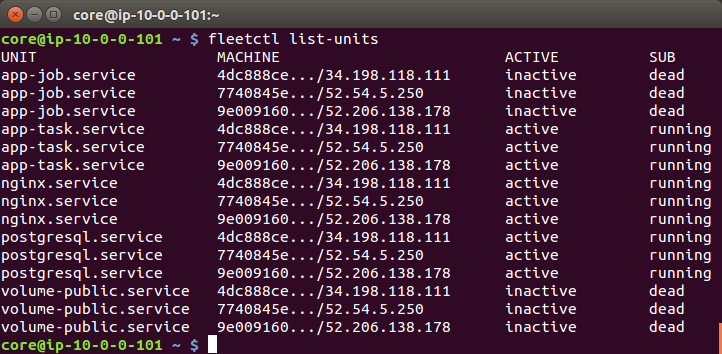
\includegraphics[width=0.8\textwidth]{images/figures/fleetctl-list-units.png}
\caption{Listado de unidades fleet en cada una de las máquinas.}
\end{figure}

Como se puede apreciar, cada una de las máquinas, con sus relativas direcciones IP, tiene una copia de cada servicio. Todas se han activado y se encuentran en ejecución, salvo las unidades \kode{app-job.service} y \kode{volume-public.service}, en particular, que aparecen inactivas porque son contenedores ejecutables, es decir, cuando acaban su cometido terminan.

También se comprueba que la actividad de la aplicación sigue siendo correcta, solicitándola con el comando \kode{curl} en cada una de las máquinas:

%= lang:bash
\begin{code}
$ for i in 1 2 3; do vagrant ssh core-0$i -c 'curl http://localhost:80 \
  | tail -n 15'; done
\end{code}

\begin{figure}[H]
\centering
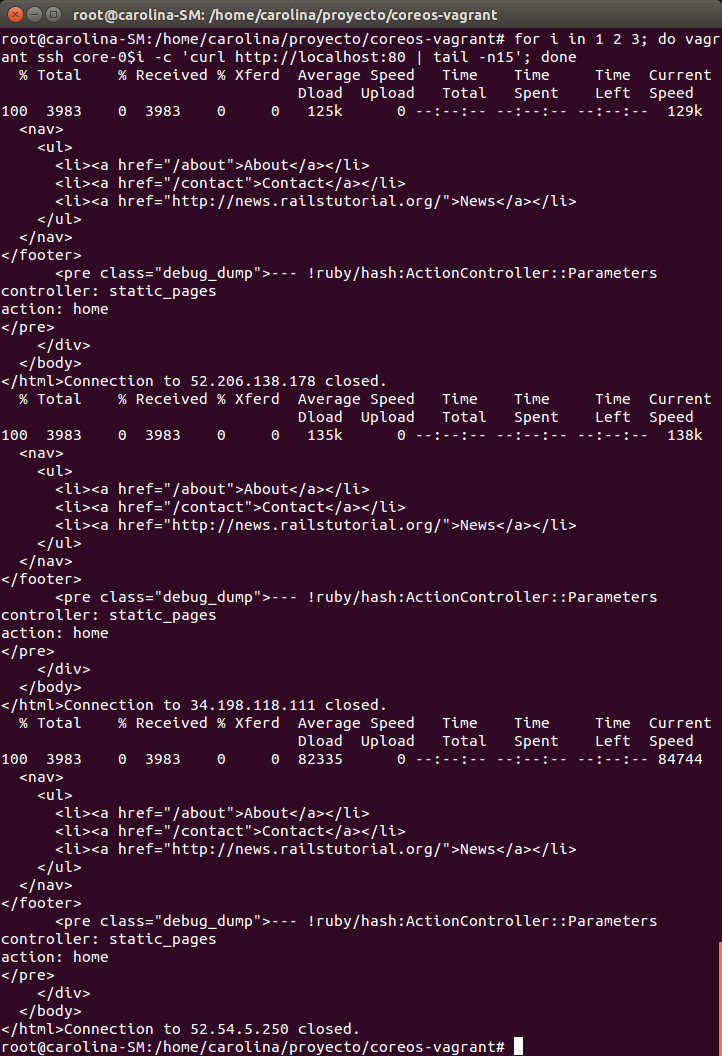
\includegraphics[width=0.75\textwidth]{images/figures/curl-fleet.png}
\caption{Acceso al servicio por consola de comandos.}
\end{figure}

\subsection{Configuración DNS usando SkyDNS}

Con el objetivo de aislar la base de datos en una sola máquina se va a hacer uso de un servidor de sistema de nombres de dominio (DNS). Es necesario puesto que los contenedores \kode{app-job}, encargado de crear, migrar y poblar la base de datos, y \kode{app-task}, el propio servicio web, necesitan acceder al contenedor \kode{some-postgres}. Este contenedor, al no estar alojado en la misma máquina, tendrá que ser registrado en el servidor DNS para que pueda ser descubierto desde las otras máquinas. Así, los contenedor \kode{app-job} y \kode{app-task} resolverán la base de datos mediante dicho servidor DNS, que tendrá presencia en todas las máquinas como un nuevo contenedor, llamado \kode{skydns}. SkyDNS es un servicio distribuido para el anuncio y descubrimiento de servicios construidos sobre etcd. De está manera crea y lee registros en él. Se trata de un proyecto de código abierto que puede ser encontrado en GitHub, bajo el repositorio \kode{skynetservices/skydns}.

Así, el primer paso consistirá en la división de la infraestructura de forma que los contenedores \kode{volume-public}, \kode{app-job}, \kode{app-task} y \kode{some-ningx} sean creados en la máquina \kode{core-01}. Por otro lado, el contenedor \kode{some-postgres} será creado en la máquina \kode{core-02}. Esto se consigue usando la opción \textit{metadata} presente en las unidades fleet. Para especificarlo es necesario añadir al fichero \kode{Vagrantfile} un metadato diferente para cada una de las máquinas, de manera que \kode{core-01} reciba \textit{compute=web} y \kode{core-02} \textit{compute=db}. Esto ha de ser añadido bajo la carga de cada una de las líneas que contiene el fichero \kode{cloud-config}.

\begin{codelisting}
\label{code:vagrantfile2}
\codecaption{Fichero \kode{Vagrantfile}}
%= lang:ruby
\begin{code}
.
data = YAML.load(IO.readlines(CLOUD_CONFIG_PATH)[1..-1].join)
if data['coreos'].key? 'fleet' and i==1
  data['coreos']['fleet']['metadata'] = 'compute=web'
end
if data['coreos'].key? 'fleet' and i==2
 data['coreos']['fleet']['metadata'] = 'compute=db'
end
.
\end{code}
\end{codelisting}

Ahora será necesario añadir el metadato a los ficheros de las unidades de servicio de los contenedores nombrados. Para la máquina \kode{core-01} el parámetro \textit{MachineMetadata=compute=web} y en el fichero correspondiente a la base de datos el parámetro \textit{MachineMetadata=compute=db}, en la máquina \kode{core-02}. Ambos en la sección \textit{[X-Fleet]}.

Como el contenedor \kode{some-postgres} ya no se encontrará en la misma máquina que el resto de contenedores no es posible compartir el volumen \kode{volume-public} con ellos. Por lo tanto se eliminará en su definición el comando \textit{-v}, que permite exportarlo, así como su inclusión en los parámentros \textit{After} y \textit{Require}.

Lo siguiente será crear el contenedor que se corresponde con el servidor DNS, presente en todas las máquinas. Este último hecho es posible no añadiendo ningún metadato en la sección \textit{[X-Fleet]}. Se escribe un nuevo fichero llamado \kode{/home/core/skydns.service} antes del fichero \kode{/home/core/volumen-public.service}. Además se le indica que será iniciado después de Docker y etcd2. Luego se procede de la misma manera que con las otras unidades de servicio. Antes de comenzar el servicio borrará el contenedor si existe previamente y luego descargará la imagen desde Docker Hub. Antes de empezar el servicio se establece la configuración de SkyDNS de forma que se especifica la dirección IP y puerto en la que debe escuchar, que será la local a la máquina por el puerto 53. También se establece el dominio para el que es autoritario, escogiéndose \kode{sampleapp.local.}, y el tiempo de vida (TTL) de las respuestas a 30 segundos. A la hora de comenzar el servicio restará indicarle que las máquinas etcd se comunican en la dirección IP privada en uso y puerto 2379. Como se trata de una unidad fleet, será necesario añadir el servicio global \kode{fleet-skydns.service} antes de \kode{fleet-volume-public.service} para comenzar el servicio. 

Así, habrá que añadir a \kode{user-data.sampleapp.aws}:

\begin{codelisting}
\label{code:user-data-skydns}
\codecaption{Fichero \kode{user-data.sampleapp.aws}}
%= lang:yaml
\begin{code}
.
write_files:
.
  - path: "/home/core/skydns.service"
    permissions: "0644"
    content: |
      [Unit]
      Description=SkyDNS
      After=docker.service etcd2.service
      Requires=docker.service etcd2.service
      [Service]
      Restart=always
      TimeoutStartSec=0
      ExecStartPre=-/usr/bin/docker rm -f skydns
      ExecStartPre=/usr/bin/docker pull skynetservices/skydns
      ExecStartPre=/usr/bin/etcdctl set /skydns/config \
        '{"dns_addr":"0.0.0.0:53", "domain": "sampleapp.local.", "ttl":30}'
      ExecStart=/usr/bin/docker run --rm --name skydns \
        -e ETCD_MACHINES="http://$private_ipv4:2379" skynetservices/skydns
      ExecStop=-/usr/bin/docker stop skydns
      [X-Fleet]
      Global=true
.
coreos:
.
  units:
  .
  - name: fleet-skydns.service
    command: start
    content: |
      [Unit]
      Description=Start skydns.service using fleet
      [Service]
      ExecStart=/usr/bin/fleetctl start /home/core/skydns.service
.
\end{code}
\end{codelisting}

Como se dijo inicialmente, este servicio funciona mediante registros y lecturas. De esta manera, al fichero \kode{/home/core/postgresql.service} hay que añadirle el registro de la dirección IP del contenedor some-postgres para que pueda ser encontrado por los otros contenedores, desde las otras máquinas. Este registro ha de ser añadido después de que el contenedor esté en ejecución, por lo que se especificará como \textit{ExecStartPost} y se llevará a cabo una espera hasta que se cumpla tal condición. Los contenedores \kode{app-job} y \kode{app-task} necesitan resolverlo como \textit{db} que es el nombre escogido como adaptador de la base de datos. Sin embargo, \kode{app-job} también resuelve por \textit{some-postgres}, puesto que antes de comenzar sus tareas espera a que dicho contenedor esté activo en el puerto 5432. Teniendo en cuenta estas condiciones se realizan dos registros, el primero tipo nombre canónico (CNAME) de \textit{some-postgres.sampleapp.local.} a \textit{db.sampleapp.local.} y el segundo tipo dirección IP (A) de \textit{db.sampleapp.local.} a dirección IP de \kode{some-postgres}, indicándole que será accesible por el puerto 5432.

\begin{codelisting}
\label{code:user-data-skydns-postgresql}
\codecaption{Fichero \kode{user-data.sampleapp.aws}}
%= lang:yaml
\begin{code}
.
write_files:
.
  - path: "/home/core/postgresql.service"
    .
      [Service]
      .
      ExecStartPost=/bin/bash -c 'while ! \
        [ $(/usr/bin/docker inspect -f ="{{.State.Running}}" some-postgres) \
        == "=true" ]; do sleep 1; done; \
        /usr/bin/etcdctl set /skydns/local/sampleapp/some-postgres \
        "{ \\"host\\": \\"db.sampleapp.local.\\"}" ; \
        /usr/bin/etcdctl set /skydns/local/sampleapp/db \
        "{ \\"host\\": \\"$(/usr/bin/docker inspect -f \
        "{{ .NetworkSettings.IPAddress }}" some-postgres)\\" , \\"port\\":5432}"'
.
\end{code}
\end{codelisting}

Referente a los contenedores \kode{app-job} y \kode{app-task} habrá que eliminar la opción \textit{---link} y utilizar las opciones \textit{---dns} que apuntará a la dirección IP del contenedor \kode{skydns} y \textit{---dns-search} donde se especifica el dominio trabajado \textit{sampleapp.local} para poder resolver por \textit{db} y \textit{some-postgres} sin especificar el dominio. La sección \textit{ExecStart} de ambas queda:

\begin{codelisting}
\label{code:user-data-skydns-app}
\codecaption{Fichero \kode{user-data.sampleapp.aws}}
%= lang:yaml
\begin{code}
.
write_files:
.
  - path: "/home/core/app-job.service"
    .
      [Service]
      .
      ExecStart=/bin/bash -c 'usr/bin/docker run --rm --name app-job \
      -v "volume-public:/usr/src/app/public" --entrypoint "./setup.sh" \
      -e "POSTGRES_USER=${POSTGRES_USER}" \
      -e "POSTGRES_PASSWORD=${POSTGRES_PASSWORD}" \
      -w "/usr/src/app" --dns $(/usr/bin/docker inspect \
      -f "{{ .NetworkSettings.IPAddress }}" skydns) \
      --dns-search "sampleapp.local" carolina/sample_app_rails_4_image:latest'
      .
  - path: "/home/core/app-task.service"
    .
      [Service]
      .
      ExecStart=/bin/bash -c 'usr/bin/docker run --rm --name app-task \
      -e "POSTGRES_USER=${POSTGRES_USER}" \
      -e "POSTGRES_PASSWORD=${POSTGRES_PASSWORD}" \
      -w "/usr/src/app" -v "volume-public:/usr/src/app/public" \
      --dns $(/usr/bin/docker inspect \
      -f "{{ .NetworkSettings.IPAddress }}" skydns) \
      --dns-search "sampleapp.local" carolina/sample_app_rails_4_image:latest \
      /bin/bash -c "cp config/database.yml.postgresql config/database.yml && \
      cp ./.secret.example ./.secret && puma -p 9292"'
      .
\end{code}
\end{codelisting}

Además habrá que quitar de las secciones \textit{After} y \textit{Requires} el servicio \kode{postgresql.service} en todos los servicios y añadir \kode{skydns.service} antes de \kode{volume-public.service} en todas las unidades de servicio.

A continuación se desplega la infraestructura:

%= lang:bash
\begin{code}
$ vagrant up --provider=aws
\end{code}

Primero se comprueba la salud del clúster, contemplada por cada máquina:

%= lang:bash
\begin{code}
$ for i in 1 2 3; do vagrant ssh core-0$i -c 'etcdctl cluster-health'; done
\end{code}

\begin{figure}[H]
\centering
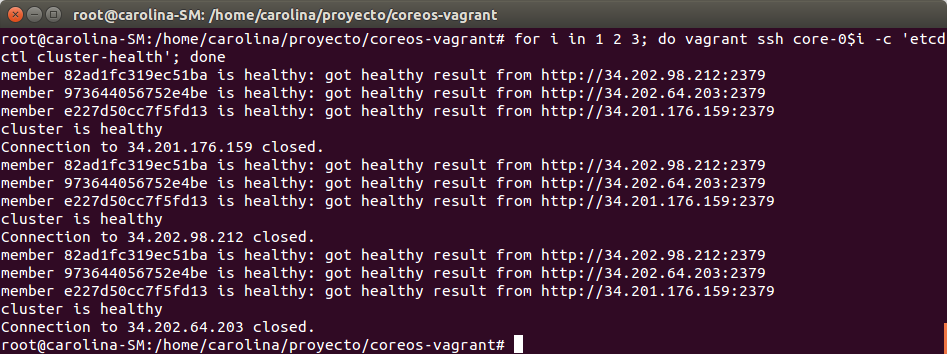
\includegraphics[width=0.8\textwidth]{images/figures/skydns-health.png}
\caption{Salud del clúster contemplada por las 3 máquinas.}
\end{figure}

Luego se listan las máquinas y se comprueba que han recibido el metadato:

%= lang:bash
\begin{code}
for i in 1 2 3; do vagrant ssh core-0$i -c 'fleetctl list-machines'; done
\end{code}

\begin{figure}[H]
\centering
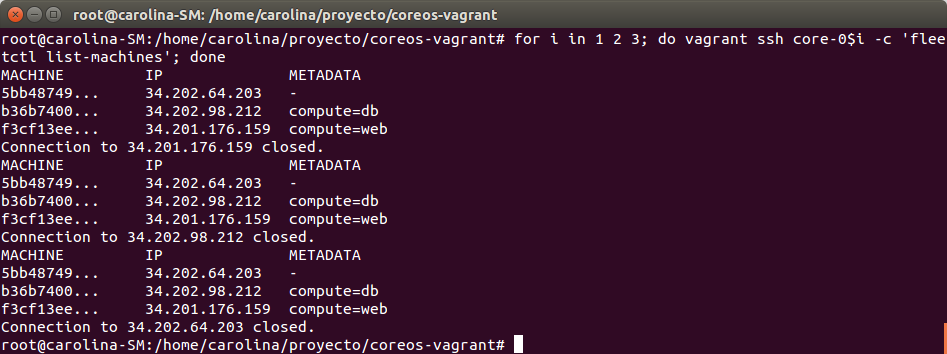
\includegraphics[width=0.8\textwidth]{images/figures/skydns-machines.png}
\caption{Información de las máquinas contemplada por las 3 máquinas.}
\end{figure}

También se comprueba que las unidades de servicio se crearon donde se indicó:
%= lang:bash
\begin{code}
$ for i in 1 2 3; do vagrant ssh core-0$i -c 'fleetctl list-units'; done
\end{code}

\begin{figure}[H]
\centering
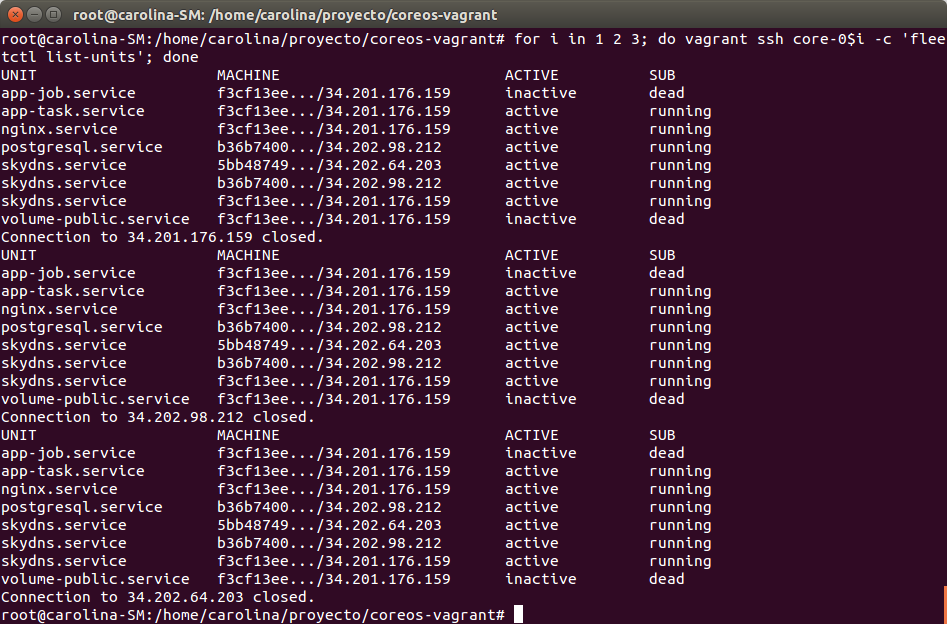
\includegraphics[width=0.8\textwidth]{images/figures/skydns-units.png}
\caption{Información de las unidades contemplada por las 3 máquinas.}
\end{figure}

Se comprueba que los registros se hayan establecido correctamente:

%= lang:bash
\begin{code}
$ for i in 1 2 3; do vagrant ssh core-0$i -c '/usr/bin/etcdctl get \
  /skydns/local/sampleapp/db; \
  /usr/bin/etcdctl get /skydns/local/sampleapp/some-postgres '; done
\end{code}

\begin{figure}[H]
\centering
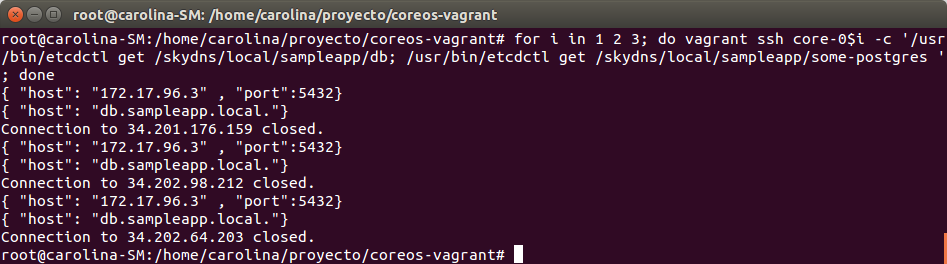
\includegraphics[width=0.9\textwidth]{images/figures/skydns-gets.png}
\caption{Lectura de los registros en SkyDNS contemplada por las 3 máquinas.}
\end{figure}

La máquina \kode{core-01} resuelve tanto \textit{db} como \textit{some-postgres}:

%= lang:bash
\begin{code}
# docker exec -it app-task sh -c 'ping -c 1 db'
# docker exec -it app-task sh -c 'ping -c 1 some-postgres'
\end{code}

\begin{figure}[H]
\centering
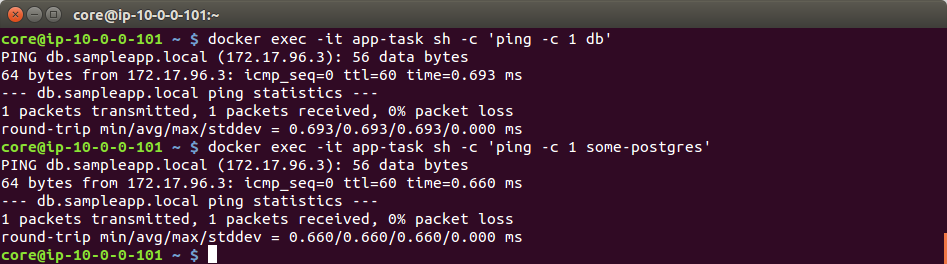
\includegraphics[width=0.9\textwidth]{images/figures/skydns-ping.png}
\caption{Conexión a \textit{db} como \textit{some-postgres} desde \kode{app-task}.}
\end{figure}

De esta manera, los registros ingresados han quedado como se pretendía:

%= lang:bash
\begin{code}
docker exec -it skydns sh -c 'dig @localhost db.sampleapp.local. A'
\end{code}

\begin{figure}[H]
\centering
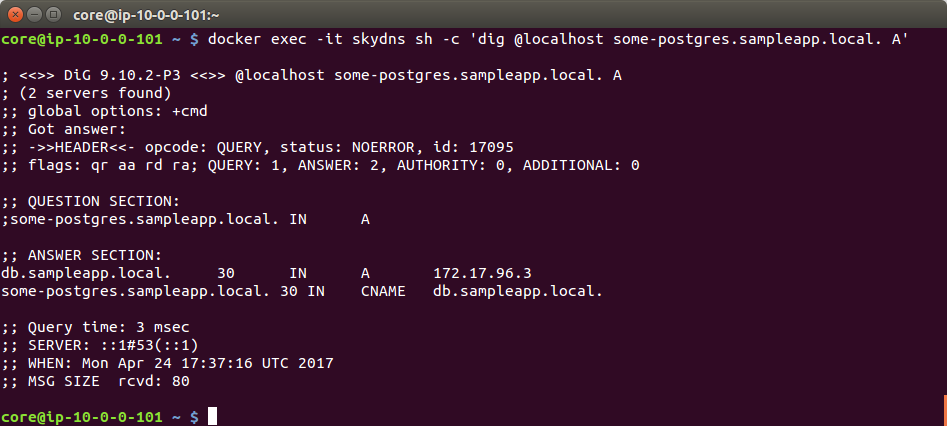
\includegraphics[width=0.85\textwidth]{images/figures/skydns-dig.png}
\caption{Registros DNS desde el contenedor \kode{skydns}.}
\end{figure}

Así, el servicio funciona correctamente en la máquina \kode{core-01}:
%= lang:bash
\begin{code}
$ for i in 1 2 3; do vagrant ssh core-0$i -c 'curl http://localhost:80 | \
  tail -n 15'; done
\end{code}

\begin{figure}[H]
\centering
\includegraphics[width=0.85\textwidth]{images/figures/skydns-curl.png}
\caption{Conexión al servicio mediante consola desde \kode{core-01}.}
\end{figure}

Y mediante la web y la dirección IP elástica se ingresa con uno de los usuarios poblados en la base de datos, comprobando que sigue funcionando correctamente hasta este punto:

\begin{figure}[H]
\centering
\includegraphics[width=0.85\textwidth]{images/figures/skydns-web.png}
\caption{Inicio de sesión con el usuario \textit{Example User} desde \kode{core-01}.}
\end{figure}

\subsection{Balanceo de carga con Nginx usando Confd}

Con el propósito de implementar la infraestructura final, en la que en cada una de las máquinas que conforma el clúster hay un servidor de la aplicación, se van a realizar una serie de cambios. En la primera máquina se sitúa el proxy, que balanceará la carga entre ellos. En la segunda máquina se encontrará la base de datos a la que acudirán los servidores de aplicación.

En primer lugar, al no encontrarse los distintos contenedores en la misma máquina la opción de tener el volumen Docker \kode{volume-public} compartido entre ellos no es posible en la manera en la que se ha ido haciendo, así que se elimina su definición en el fichero \kode{user-data.sampleapp.aws}, en \kode{/home/core/volume-public.service}, su inclusión en los parámetros \textit{After} y \textit{Requires} en los servicios que lo implementan, el parámetro \textit{-v} que lo exporta en los contenedores \kode{app-job}, \kode{app-task} y \kode{some-nginx}, así como la unidad global \kode{fleet-volume-public.service}.

El despliegue de la infraestructura será controlado, una vez más, con metadatos. Para ello se mantiene a la máquina \kode{core-02} con el metadato \textit{compute=db} y se modifica en el fichero \kode{Vagrantfile}, bajo la carga de la línea que contiene la sección de configuración fleet en el fichero \kode{user-data}, el metadato para la máquina \kode{core-01}, cambiándolo por \textit{compute=proxy}.

\begin{codelisting}
\label{code:vagrantfile2}
\codecaption{Fichero \kode{Vagrantfile}}
%= lang:ruby
\begin{code}
.
data = YAML.load(IO.readlines(CLOUD_CONFIG_PATH)[1..-1].join)
if data['coreos'].key? 'fleet' and i==1
 data['coreos']['fleet']['metadata'] = 'compute=proxy'
end
.
\end{code}
\end{codelisting}

Ahora será necesario modificar el metadato de la unidad de servicio \kode{postgresql.service} a \textit{MachineMetadata=compute=proxy}, en la sección \textit{[X-Fleet]}. Además, se quita  en las unidades de servicio \kode{app-job.service} y \kode{app-task.service}, para que sean ubicadas en cada máquina.

En este caso se supone que siempre quiere tenerse el servidor web \kode{app-task} activo en cada máquina, así que se prepara para que en caso de fallo vuelva a activarse. Esto se consigue con el parámetro \textit{Restart=always}.

Como el servicio \kode{nginx.service} tendrá que balancear la carga entre los distintos servidores web disponibles, será necesario que el servidor \kode{app-task} se registre tras crearse. Este registro se va a realizar en etc2, por lo tanto, éste se añade en los parámetros \textit{After} y \textit{Requires} como \kode{etcd2.service} tras \kode{docker.service}. Así, el registro se añade en la sección \textit{ExecStartPost} con clave \kode{/services/app/<dirección IP de la máquina en la que se encuentra>} y valor correspondiente con la dirección IP del contenedor y puerto 9292, pues se hace referencia al servidor puma. Esto permitirá tener tantas entradas \kode{/services/app/*} como máquinas en las que se ejecute hayan. Es importante añadir que cuando el contenedor deje de ejecutarse dicho registro sea borrado. Para interpretar la dirección IP de la máquina es necesario indicar el fichero de variables de entorno \kode{/etc/environment}. 

\begin{codelisting}
\label{code:execstartpost-app-task}
\codecaption{Fichero \kode{user-data.sampleapp.aws}}
%= lang:yaml
\begin{code}
.
write_files:
.
  - path: "/home/core/app-task.service"
    .
    [Service] 
      .
      Restart=always     
      EnvironmentFile=/etc/environment
      .
      ExecStartPost=/bin/bash -c 'while ! [ $(/usr/bin/docker inspect \
      -f ="{{.State.Running}}" app-task) == "=true" ]; do sleep 1; done; \
      etcdctl set /services/app/${COREOS_PRIVATE_IPV4} $(/usr/bin/docker \
      inspect -f "{{ .NetworkSettings.IPAddress }}" app-task):9292'
      ExecStop=/usr/bin/etcdctl rm /services/app/${COREOS_PRIVATE_IPV4}
      .
.
\end{code}
\end{codelisting}

Para que el servicio \kode{nginx.service} pueda registrar los servidores web puma se va a utilizar el servicio confd. Esta utilidad se encarga de controlar los cambios que se produzcan en etc2, vigilando las claves que se le indique. Cuando hay un nuevo registro o baja transfiere estos cambios a la configuración de nginx, por medio de una plantilla, modificando el fichero \kode{/etc/nginx.conf} del contenedor \kode{some-nginx}. Luego, hace efectivo el cambio reiniciando el servicio nginx. Este servicio puede ser encontrado en el repositorio \kode{kelseyhightower/confd} en GitHub, del que se hará una configuración especifica para este uso.

Como se pretende compartir el fichero de configuración \kode{nginx.conf} entre el contenedor \kode{some-nginx} y el futuro contenedor \kode{confd} se crea un volumen Docker, llamado \kode{conf-data}, que compartirá el directorio \kode{/etc/nginx} entre ambos. En su definición se indica requiere y ha de ser lanzado después del servicio \kode{docker.service}. Se indica que el servicio será de tipo \textit{oneshot}, lo que significa que el parámetro \textit{ExecStart} ha de ejecutarse solo una vez, sin reintentarlo. También se especifica la opción \textit{RemainAfterExit=yes} para que cuando el contenedor termine permanezca activo. Si el volumen existe en su lanzamiento se detiene y elimina. La imagen que se usa para el contenedor es la de nginx, para poder tener la misma disposición de directorios. Este volumen deberá ubicarse en la máquina \kode{core-01}, por lo que se le añade el metadato \kode{compute=proxy}. Además. será necesario crear la unidad global \kode{fleet-conf-data.service} que de comienzo a este servicio fleet.

\begin{codelisting}
\label{code:conf-data}
\codecaption{Fichero \kode{user-data.sampleapp.aws}}
%= lang:yaml
\begin{code}
.
write_files:
.
  - path: "/home/core/conf-data.service"
    permissions: "0644"
    content: |
      [Unit] 
      Description=conf data container to share files between confd and some-nginx
      After=docker.service
      Requires=docker.service
      [Service] 
      Type=oneshot
      RemainAfterExit=yes
      ExecStartPre=-/usr/bin/docker kill conf-data 
      ExecStartPre=-/usr/bin/docker rm conf-data
      ExecStartPre=/usr/bin/docker pull nginx 
      ExecStart=/usr/bin/docker run -v /etc/nginx --name conf-data nginx \
      echo "conf-data container created" 
      [X-Fleet]
      Global=true
      MachineMetadata=compute=proxy
  .
coreos:
  .
  units:
  .
  - name: fleet-conf-data.service
    command: start
    content: |
      [Unit]
      Description=Start conf-data.service using fleet
      [Service]
      ExecStart=/usr/bin/fleetctl start /home/core/conf-data.service
  .
\end{code}
\end{codelisting}

El servicio confd necesitará disponer de tres ficheros, que serán escritos en la máquina y exportados al contenedor a través del volumen \kode{conf-data}.

El primero de ellos es la plantilla \kode{nginx.conf.tmpl}, correspondiente a la configuración de nginx. Al incorporarlo a \kode{user-data.sampleapp.app} puede borrarse la definición del fichero \kode{/etc/nginx.conf}, presente en la sección \textit{write-files}. La información a añadir es el bloque \textit{upstream} utilizado para definir los servidores web. Nginx seleccionará uno de ellos dependiendo del método de distribución escogido, en este caso \textit{Round Robin}, del primero al último, que por defecto es el que se implementa. Mediante una plantilla en formato \textit{Go}, que permite gestionar contenido dinámico, se define este nuevo bloque, que ha de estar, a su vez, dentro del bloque \textit{http} y requiere la existencia del bloque \textit{events} para gestionar eventos, aunque no sea utilizado. Así, cuando confd analice etc2 en busca de cambios para las claves \kode{/services/app/*} sustituirá dinámicamente su contenido por las líneas \textit{server <dirección IP del contenedor \kode{app-task}>:9292}, en lugar de tener que definirlos estáticamente. El servidor escogido pasará a \textit{proxy\_pass http://app;}.

\begin{codelisting}
\label{code:nginx.conf.tmpl}
\codecaption{Fichero \kode{user-data.sampleapp.aws}}
%= lang:yaml
\begin{code}
.
write_files:
.
  - path: "/etc/nginx.conf.tmpl"
    permissions: "0644"
    content: |
      events {
      }
      http {
        upstream app {
        {{ range getvs "/services/app/*" }}
          server {{ . }};
        {{ end }}
        }

        server {
          listen 80;
          root /usr/src/app/public;
          location / {
            proxy_set_header X-Forwarded-For $proxy_add_x_forwarded_for;
            proxy_set_header Host $http_host;
            proxy_redirect off;
            try_files $uri /page_cache/$uri /page_cache/$uri.html @app;
          }
          location @app{
            proxy_pass http://app;
            break;
          }
        }
      }
.
\end{code}
\end{codelisting}

El siguiente, llamado \kode{nginx.toml}, representa el fichero de configuración confd. Está escrito en formato TOML, comprueba el valor de las claves registradas bajo \kode{/services/app} y realiza la acción del cambio del archivo \kode{/etc/nginx/nginx.conf}, tomando como fuente la plantilla anterior, \kode{nginx.conf.tmpl}. El servicio confd ha de encargarse de reiniciar el servicio Nginx. Para ello ejecuta el fichero \kode{/reload.sh} que permitirá ejecutar una orden, mediante el comando curl, haciendo uso del socket de Docker, puesto que éste no estará instalado en el contenedor \kode{confd}. Esta orden hará que capture el identificador del contenedor \kode{some-nginx}, a través del lenguaje de gestión de flujos de datos JSON \textit{jq}, y detenga el proceso. 

\begin{codelisting}
\label{code:nginx.conf.tmpl}
\codecaption{Fichero \kode{user-data.sampleapp.aws}}
%= lang:yaml
\begin{code}
.
write_files:
.
  - path: "/home/core/reload.sh"
    permissions: "0644"
    content: |
      #!/bin/sh
      curl --unix-socket /var/run/docker.sock -XPOST \
      "http://v1.26/containers/$(curl --unix-socket /var/run/docker.sock \
      'http://v1.26/containers/json' | jq -r '.[] | \
       select(.Names[0] == "/some-nginx") .Id')/kill"
  - path: "/etc/nginx.toml"
    permissions: "0644"
    content: |
      [template]
      src = "nginx.conf.tmpl"
      dest = "/etc/nginx/nginx.conf"
      keys = [ "/services/app" ] 
      reload_cmd = "sh /reload.sh"
.
\end{code}
\end{codelisting}

Para disponer de una imagen Docker propia de confd se crea una nueva, llamada \kode{confd\_image}, a partir del fichero Dockerfile. Se utiliza una imagen \textit{Alpine Linux}\footnotettt{Alpine Linux}{https://www.alpinelinux.org/about} con un índice de paquetes completo y solo 5 MB de tamaño, en su versión 3.3. Sobre esta imagen se instalarán los paquetes \textit{curl}, para hacer la recarga del servicio, y el \textit{jq}, para obtener el identificador del contenedor \kode{some-nginx}. Luego se obtiene la herramienta confd para sistemas Linux con CPUs AMD de 64 bits, se le dan permisos de lectura, escritura y ejecución al propietario en \kode{/usr/bin/confd} para poder realizar operaciones y se limpia la memoria caché utilizada. Además, se añade el directorio vacío \kode{/etc/confd} que será utilizado para alojar los ficheros. Por último, se indica que una vez arrancado un contenedor con esta imagen, el servicio confd vigilará los cambios producidos en etc2, en todo el clúster, cada 5 segundos.

\begin{codelisting}
\label{code:dockerfile-confd}
\codecaption{Contenido de \kode{Dockerfile}}
%= lang:ruby
\begin{code}
FROM alpine:3.3
LABEL confd_image.version="0.1" confd_image.release-date="2017-05-02"
MAINTAINER Carolina Santana "c.santanamartel@gmail.com"
RUN apk add --update curl && apk add --update jq && \
    curl -o /usr/bin/confd -L https://github.com/kelseyhightower/confd/releases/
            download/v0.7.1/confd-0.7.1-linux-amd64 && \
    chmod 755 /usr/bin/confd && rm -rf /var/cache/apk/*
ADD etc/confd/ /etc/confd
CMD /usr/bin/confd -interval=5 -node=http://$COREOS_PRIVATE_IPV4:4001
\end{code}
\end{codelisting}

De esta manera, será necesario crear en local el directorio vacío \kode{etc/confd}, construir la imagen y subirla a Docker Hub para poder usarla:

%= lang:bash
\begin{code}
$ mkdir etc/confd
$ docker login
$ docker build -t confd_image .
$ docker tag <image-id> carolina/confd_image:latest
$ sudo docker push carolina/confd_image
\end{code}

Cuando el proceso de subida ha terminado, se define el fichero \kode{/home/core/confd.service} que creará el contenedor \kode{confd}. Así, requiere y ha de ser creado tras los servicios \kode{docker.service}, \kode{etcd2.service}, pues leerá de él, y \kode{conf-data.service}. Se indica que comience automáticamente los intentos de ejecución de \textit{ExecStart} y se añade el fichero de variables de entorno \kode{/etc/environment} para que pueda conocer las direcciones IP de las máquinas que conforman el clúster. Si en el momento de ser lanzado ya existiera se manda a detener el proceso y se elimina el contenedor. Antes de crearlo se descarga la última versión de la imagen \kode{confd\_image}, si no se tiene. Además de pasarle la variable de entorno comentada, se exporta el \textit{socket} de Docker, para poder usarlo a la hora de ejecutar la recarga del servicio nginx y los tres archivos escritos, donde los destinos finales serán \kode{/etc/confd/templates/nginx.conf.tmpl}, \kode{/reload.sh} y \kode{/etc/confd/conf.d/nginx.toml}. Por último se añade el volumen \kode{conf-data}. Este contenedor deberá ubicarse en la máquina \kode{core-01}, por lo que se le añade el metadato \kode{compute=proxy}. También se crea la unidad global \kode{fleet-confd.service} que comienza este servicio.

\begin{codelisting}
\label{code:confd}
\codecaption{Fichero \kode{user-data.sampleapp.aws}}
%= lang:yaml
\begin{code}
.
write_files:
.
  - path: "/home/core/confd.service"
    permissions: "0644"
    content: |
      [Unit] 
      Description=confd container that updates nginx.conf file and kill 
                  some-nginx container to restart nginx service when detects
                  a new rails server has been registered
      After=docker.service etcd2.service conf-data.service
      Requires=docker.service etcd2.service conf-data.service
      [Service] 
      TimeoutStartSec=0 
      EnvironmentFile=/etc/environment
      ExecStartPre=-/usr/bin/docker kill confd 
      ExecStartPre=-/usr/bin/docker rm confd
      ExecStartPre=/usr/bin/docker pull carolina/confd_image:latest 
      ExecStart=/bin/bash -c '/usr/bin/docker run --rm --name confd \
      -e COREOS_PRIVATE_IPV4=${COREOS_PRIVATE_IPV4} \
      -v "/var/run/docker.sock:/var/run/docker.sock" \
      -v "/etc/nginx.conf.tmpl:/etc/confd/templates/nginx.conf.tmpl" \
      -v "/home/core/reload.sh:/reload.sh" \
      -v "/etc/nginx.toml:/etc/confd/conf.d/nginx.toml" \
      --volumes-from=conf-data carolina/confd_image '
      ExecStop=/usr/bin/docker stop confd
      [X-Fleet]
      Global=true
      MachineMetadata=compute=proxy
  .
coreos:
  .
  units:
  .
  - name: fleet-confd.service
    command: start
    content: |
      [Unit]
      Description=Start confd.service using fleet
      [Service]
      ExecStart=/usr/bin/fleetctl start /home/core/confd.service
  .
\end{code}
\end{codelisting}

En último lugar se modifica el fichero \kode{/home/core/nginx.service} de manera que se especifique en las opciones \textit{After} y \textit{Requires} que requiere y ha de ir tras los servicios \kode{docker.service}, \kode{conf-data.service} y \kode{confd.service}. Como el servicio confd se encargará de detener el proceso de \kode{some-nginx} se añade la opción \textit{Restart=always} que hará que la unidad de servicio vuelva a ejecutarse con la nueva configuración Nginx. Además, en la creación del contenedor, \textit{ExecStart}, se elimina la opción \kode{--link app-task:app} y el fichero de configuración que se exportaba anteriormente \kode{-v /etc/nginx.conf:/etc/nginx/nginx.conf} y se añade la opción \kode{--volumes-from=conf-data}.

A continuación se despliega la infraestructura:

%= lang:bash
\begin{code}
$ . ~/.aws-credentials/aws-credentials && vagrant up --provider=aws
\end{code}

En primer lugar se comprueba la salud del clúster:

%= lang:bash
\begin{code}
$ for i in 1 2 3; do vagrant ssh core-0$i -c 'etcdctl cluster-health'; done
\end{code}

\begin{figure}[H]
\centering
\includegraphics[width=0.75\textwidth]{images/figures/health-confd.png}
\caption{Salud del clúster contemplada por las 3 máquinas.}
\end{figure}

También, se visualizan las máquinas que conforman el clúster, con los metadatos asignados y las unidades fleet presentes en cada máquina:

%= lang:bash
\begin{code}
$ for i in 1 2 3; do vagrant ssh core-0$i -c 'fleetctl list-machines'; done
\end{code}

\begin{figure}[H]
\centering
\includegraphics[width=0.75\textwidth]{images/figures/machines-confd.png}
\caption{Información de las máquinas contemplada por las 3 máquinas.}
\end{figure}

%= lang:bash
\begin{code}
$ for i in 1 2 3; do vagrant ssh core-0$i -c 'fleetctl list-units'; done
\end{code}

\begin{figure}[H]
\centering
\includegraphics[width=0.65\textwidth]{images/figures/units-confd.png}
\caption{Información de las unidades fleet contemplada por las 3 máquinas.}
\end{figure}

Para continuar con las pruebas se escoge la máquina \kode{core-01}.

Se comprueban los registros existentes bajo la clave \kode{services/app/<dirección IP de \kode{app-task}>}. Las claves se averiguan con el comando \kode{etcdctl ls --recursive /services/app} y luego los valores con el comando \kode{etcdctl get /services/app/<dirección IP de \kode{app-task}>}:

\begin{figure}[H]
\centering
\includegraphics[width=0.7\textwidth]{images/figures/recursive-confd.png}
\caption{Obtención de claves y valores para \kode{services/app/*}.}
\end{figure}

Ahora que los contenedores \kode{app-task} se han registrado se comprueba que el servicio confd ha actualizado el fichero de configuración Nginx, a medida que los ha ido detectando. Esto es observado desde los registros de operación del servicio \kode{confd.service} y dentro del contenedor \kode{some-nginx}, viendo el contenido del fichero \kode{/etc/nginx/nginx.conf}:

%= lang:bash
\begin{code}
# journalctl -u confd.service
\end{code}

\begin{figure}[H]
\centering
\includegraphics[width=0.75\textwidth]{images/figures/update-journal-confd.png}
\caption{Actualización de la configuración Nginx desde \kode{confd}.}
\end{figure}

%= lang:bash
\begin{code}
# docker exec -it some-nginx sh
# cat /etc/nginx/nginx.conf
\end{code}

\begin{figure}[H]
\centering
\includegraphics[width=0.6\textwidth]{images/figures/update-nginx-confd.png}
\caption{Fichero \kode{nginx.conf} actualizado.}
\end{figure}

Tras ver el orden en el que se han colocado las distintas direcciones IP de los contenedores \kode{app-task} puede conocerse de qué máquina proviene cada uno inspeccionando el contenedor en cada máquina:

%= lang:bash
\begin{code}
$ docker inspect app-task -f "{{ .NetworkSettings.IPAddress }}"
\end{code}

\begin{figure}[H]
\centering
\includegraphics[width=0.8\textwidth]{images/figures/IP1-confd.png}
\caption{Dirección IP del contenedor \kode{app-task} en la máquina \kode{core-01}.}
\end{figure}

\begin{figure}[H]
\centering
\includegraphics[width=0.8\textwidth]{images/figures/IP2-confd.png}
\caption{Dirección IP del contenedor \kode{app-task} en la máquina \kode{core-02}.}
\end{figure}

\begin{figure}[H]
\centering
\includegraphics[width=0.8\textwidth]{images/figures/IP3-confd.png}
\caption{Dirección IP del contenedor \kode{app-task} en la máquina \kode{core-03}.}
\end{figure}

Por lo tanto el orden establecido ha sido: \kode{core-03}, \kode{core-01} y \kode{core-02}.

Así mismo, si se realizan 3 peticiones de servicio prácticamente juntas, desde la máquina \kode{core-01} en el que se encuentra el proxy, se puede comprobar por la hora marcada como las peticiones se envían en dicho orden.

%= lang:bash
\begin{code}
$ for i in 1 2 3; do curl http://localhost:80 | tail -n 15; done
\end{code}

Para comprobar cuándo fueron resueltas las peticiones se ejecuta:

%= lang:bash
\begin{code}
$ docker logs app-task
\end{code}

\begin{figure}[H]
\centering
\includegraphics[width=0.7\textwidth]{images/figures/logs3-confd.png}
\caption{Información de \kode{app-task} sobre una petición en \kode{core-03}.}
\end{figure}

\begin{figure}[H]
\centering
\includegraphics[width=0.7\textwidth]{images/figures/logs1-confd.png}
\caption{Información de \kode{app-task} sobre una petición en \kode{core-01}.}
\end{figure}

\begin{figure}[H]
\centering
\includegraphics[width=0.7\textwidth]{images/figures/logs2-confd.png}
\caption{Información de \kode{app-task} sobre una petición en \kode{core-02}.}
\end{figure}

Finalmente se visualiza el servicio, siendo balanceada la carga entre los distintos servidores web de forma transparente al usuario.

\begin{figure}[H]
\centering
\includegraphics[width=0.6\textwidth]{images/figures/curl-confd.png}
\caption{Respuesta al servicio por comandos en \kode{core-01}.}
\end{figure}

\begin{figure}[H]
\centering
\includegraphics[width=0.6\textwidth]{images/figures/web-confd.png}
\caption{Respuesta al servicio por el navegador web en \kode{core-01}.}
\end{figure}

Además se inicia sesión con uno de los usuarios con los que se ha alimentado la base de datos para comprobar el correcto funcionamiento de las solicitudes a la base de datos desde esta infraestructura. El usuario a usar es \textit{example@railstutorial.org} y la contraseña \textit{foobar}:

\begin{figure}[H]
\centering
\includegraphics[width=0.7\textwidth]{images/figures/login-confd.png}
\caption{Inicio de sesión en el servicio con el usuario \textit{Example User}.}
\end{figure}

Haciendo una escritura desde el mismo servidor que ha iniciado la sesión:

\begin{figure}[H]
\centering
\includegraphics[width=0.7\textwidth]{images/figures/post-confd.png}
\caption{Escritura de un comentario con el usuario \textit{Example User}.}
\end{figure}

La información sobre las instancias puede ser consultada desde la consola de AWS:

\begin{figure}[H]
\centering
\includegraphics[width=0.8\textwidth]{images/figures/aws-confd.png}
\caption{Visualización de las instancias desde la consola de AWS.}
\end{figure}

\subsection{Resultado}

En esta iteración se ha conseguido el despliegue de la aplicación distribuida en un clúster, compuesto de tres instancias, en la nube pública de Amazon Web Services.

De esta manera se posee una infraestructura con servicios web de la aplicación replicados en una o tantas instancias como existan en el clúster, apreciando la característica de redundancia. 

Además, el proxy dispone de la opción de balanceo de carga con el uso del servicio confd, que controla los nuevos registros o bajas de los servidores web y actualiza el fichero de configuración Nginx para que pueda resolver hacia ellos. 

Con el clúster constituido sobre la nube pública de AWS, permitiendo mantener los servicios basados en contenedores, así como las máquinas monitorizadas entre sí, también está presente la alta disponibilidad de servicios. De esta forma, la configuración establecida responde ante el fallo de una unidad o máquina, recargándola para volver a ofrecer correctamente el servicio.

El correcto funcionamiento del servicio web de la aplicación quedará disponible mediante el despliegue de la infraestructura desde Vagrant, estableciendo las variables de entorno correspondientes al proveedor. La manera de proceder es accediendo directamente por el proxy, en la máquina \kode{core-01}:

%= lang:bash
\begin{code}
$ . ~/.aws-credentials/aws-credentials
$ vagrant up --provider=aws
$ vagrant ssh core-01
# curl http://localhost:80
\end{code}

\begin{figure}[H]
\centering
\includegraphics[width=0.65\textwidth]{images/figures/web-confd.png}
\caption{Respuesta al servicio por el navegador web en \kode{core-01}.}
\end{figure}

A su vez, se replica la infraestructura final para el proveedor VirtualBox, reemplazando el contenido del fichero \kode{user-data.sampleapp.vbox} por el de \kode{user-data.sampleapp.aws}, manteniendo la interfaz de flannel como pública y la red virtual 10.1.0.0/16. En el fichero \kode{Vagrantfile} se pasarían a parte común la adición de los metadatos a las máquinas.

En este caso el despliegue será de la siguiente manera:

%= lang:bash
\begin{code}
$ vagrant up 
\end{code}

Cuando el despliegue termina se comprueba la salud positiva del clúster:

%= lang:bash
\begin{code}
$ for i in 1 2 3; do vagrant ssh core-0$i -c 'etcdctl cluster-health'; done
\end{code}

\begin{figure}[H]
\centering
\includegraphics[width=0.7\textwidth]{images/figures/health-vbox.png}
\caption{Salud del clúster contemplada por las 3 máquinas.}
\end{figure}

También se obtienen las máquinas que componen el clúster desde la máquina \kode{core-03} y las unidades de servicio desde \kode{core-02}, como prueba de que se está implementando la infraestructura final:

%= lang:bash
\begin{code}
$ vagrant ssh core-03
# fleetctl list-machines
\end{code}

\begin{figure}[H]
\centering
\includegraphics[width=0.7\textwidth]{images/figures/machines-vbox.png}
\caption{Información de las máquinas del clúster.}
\end{figure}

%= lang:bash
\begin{code}
$ vagrant ssh core-02
# fleetctl list-units
\end{code}

\begin{figure}[H]
\centering
\includegraphics[width=0.7\textwidth]{images/figures/units-vbox.png}
\caption{Información de las unidades de servicio del clúster.}
\end{figure}

Por último, se replican en VirtualBox cada una de las pruebas realizadas para el proveedor AWS, confirmando el correcto funcionamiento del servicio de la aplicación y balanceo de carga entre los diferentes servidores web. Así, se muestra el correcto resultado de una petición desde \kode{core-01}:

%= lang:bash
\begin{code}
$ vagrant ssh core-01
# curl http://localhost:80 | tail -n 15
\end{code}

\begin{figure}[H]
\centering
\includegraphics[width=0.7\textwidth]{images/figures/curl-vbox.png}
\caption{Acceso al servicio desde \kode{core-01}.}
\end{figure}

El resultado final está presentado en los siguientes repositorios GitHub:
\begin{itemize}
\item \kode{CarolinaSantana/sample\_app\_rails\_4-1}: a partir del que se construye la imagen de la aplicación.
\item \kode{CarolinaSantana/coreos-vagrant}: Infraestructura como Código a desplegar en los proveedores VirtualBox o Amazon Web Services.
\end{itemize}
